%% 代码没有生成 fig_5_a-f_1.pdf, fig_1_d.pdf ?
%% Copyright 2007-2019 Elsevier Ltd
%% 
%% This file is part of the 'Elsarticle Bundle'.
%% ---------------------------------------------
%% 
%% It may be distributed under the conditions of the LaTeX Project Public
%% License, either version 1.2 of this license or (at your option) any
%% later version.  The latest version of this license is in
%%    http://www.latex-project.org/lppl.txt
%% and version 1.2 or later is part of all distributions of LaTeX
%% version 1999/12/01 or later.
%% 
%% The list of all files belonging to the 'Elsarticle Bundle' is
%% given in the file `manifest.txt'.
%% 

%% Template article for Elsevier's document class `elsarticle'
%% with numbered style bibliographic references
%% SP 2008/03/01
%%
%% 
%%
%% $Id: elsarticle-template-num.tex 168 2019-02-25 07:15:41Z apu.v $
%%
%%
%\documentclass[preprint,12pt]{elsarticle}
%\documentclass[final,1p,times,twocolumn]{elsarticle} 
\documentclass[final,3p,times,twocolumn]{elsarticle}
%% Use the option review to obtain double line spacing
%% \documentclass[authoryear,preprint,review,12pt]{elsarticle}

%% Use the options 1p,twocolumn; 3p; 3p,twocolumn; 5p; or 5p,twocolumn
%% for a journal layout:
%% \documentclass[final,1p,times]{elsarticle}
% \documentclass[final,1p,times,twocolumn]{elsarticle}
%% \documentclass[final,3p,times]{elsarticle}
%% \documentclass[final,3p,times,twocolumn]{elsarticle}
%% \documentclass[final,5p,times]{elsarticle}
%% \documentclass[final,5p,times,twocolumn]{elsarticle}

%% For including figures, graphicx.sty has been loaded in
%% elsarticle.cls. If you prefer to use the old commands
%% please give \usepackage{epsfig}

%% The amssymb package provides various useful mathematical symbols
\usepackage{amssymb}
%% The amsthm package provides extended theorem environments
%% \usepackage{amsthm}

%% The lineno packages adds line numbers. Start line numbering with
%% \begin{linenumbers}, end it with \end{linenumbers}. Or switch it on
%% for the whole article with \linenumbers.
%% \usepackage{lineno}

\graphicspath{{image/}}
\usepackage{float}
\usepackage{caption}
\usepackage{array}
\usepackage{booktabs}
 % 设置超链接跳转
\usepackage[colorlinks,
            linkcolor=blue,
            anchorcolor=blue,
            citecolor=blue]{hyperref} 
\usepackage{amsmath}

% 改变字体颜色
\usepackage{color,xcolor}
\usepackage{makecell}

% 智能引用
\usepackage{hyperref}
\usepackage{cleveref}
%
%% 跨文件引用
\usepackage{xr}
\externaldocument{figs/prediction_accuracies}

% include文件不分页
%\usepackage{newclude}

% 给表格添加注脚
\usepackage{threeparttable}
\usepackage{footnote}

% plot subfigure
\usepackage{graphicx}
\usepackage{subfigure}

% degree
\usepackage{gensymb}


\journal{Neurocomputing}

\begin{document}

\begin{frontmatter}

%% Title, authors and addresses

%% use the tnoteref command within \title for footnotes;
%% use the tnotetext command for theassociated footnote;
%% use the fnref command within \author or \address for footnotes;
%% use the fntext command for theassociated footnote;
%% use the corref command within \author for corresponding author footnotes;
%% use the cortext command for theassociated footnote;
%% use the ead command for the email address,
%% and the form \ead[url] for the home page:
%% \title{Title\tnoteref{label1}}
%% \tnotetext[label1]{}
%% \author{Name\corref{cor1}\fnref{label2}}
%% \ead{email address}
%% \ead[url]{home page}
%% \fntext[label2]{}
%% \cortext[cor1]{}
%% \address{Address\fnref{label3}}
%% \fntext[label3]{}

% Brain-like Auditory Network
\title{BAN: Neuroanatomical Aligning in Face Detection between \\Deep Neural Network and Human Brain}

%% use optional labels to link authors explicitly to addresses:
 \author[label1]{Haidong Wang}
 \ead{haidong@hnu.edu.cn}
 \author[label1]{Zhiyong Li\corref{cor1}}
 \ead{zhiyong.li@hnu.edu.cn}
 \author[label1]{Ke Nai}
 \ead{naike\_hnu@hnu.edu.cn}
 \author[label1]{Jin Yuan}
 \ead{yuanjin@hnu.edu.cn}
 \author[label2]{Shutao Li}
 \ead{shutao\_li@hnu.edu.cn}
 \author[label3]{Xianghua Li}
 \ead{493630379@qq.com}
 \address[label1]{College of Computer Science and Electronic Engineering, Hunan University, Changsha, China}
 \address[label2]{College of Electrical and Information Engineering, Hunan University, Changsha, China}
 \address[label3]{State Grid Hunan Electric Power Company Limited Economical and Technical Research Institute, Changsha, China}
\cortext[cor1]{Corresponding authors.}

%\author{}
%
%\address{}

\begin{abstract}
Inspired by neuroanatomy, deep neural networks (DNNs) have recently developed from shallow network structures to exceedingly deep structures, providing excellent recognition performance.
However, standard DNNs usually do not easily connect with brain areas on account of their excessive network depth and absent biological constraints, such as recurrent connections. 
We propose a brain-like auditory network (BAN) with four neuroanatomically mapped regions and recurrence, guided by the brain-like auditory score (BAS), 
a novel benchmark to measure the model similarity of the human smooth pursuit pathway. 
In addition, we propose that the middle temporal (MT) and medial superior temporal (MST) areas in the cerebral cortex are equivalent to the designed network structure on the basis of the continuous motion perception of the tracking pathway, 
and indicate that the metrics between the neuroanatomical similarity in the cerebral cortex and visual tracking of the DNN are compatible. 
Despite having significant tracking performance on the Tracking-Gump dataset, the BTN has achieved a high BTS. 
In summary, this research builds a BTN, a brain-like and recurrent DNN, as the first model of the cortical pathway of smooth pursuit.
\end{abstract}


\begin{keyword}
%% keywords here, in the form: keyword \sep keyword

%% PACS codes here, in the form: \PACS code \sep code

%% MSC codes here, in the form: \MSC code \sep code
%% or \MSC[2008] code \sep code (2000 is the default)
Visual object tracking \sep deep neural network \sep neuroscience \sep smooth pursuit

\end{keyword}

\end{frontmatter}

%% \linenumbers

\begin{figure*}
	\centering
	\includegraphics[width=6.7in]{figs/introduction.pdf}
	\caption{
		\textbf{
		Collaborative design between a DNN and neuroanatomy with a BTS.} 
		Through the quantitative brain-like score, we refer to the human brain and utilize acquired knowledge to enlighten the design of the BTN. 
		The BTN includes four regions that are mapped into the 		primary visual cortex (V1), 
		the middle temporal and medial superior temporal areas (MT/MST), the frontal eye field (FEF) and the brainstem/cerebellum. 
		CONV\textsubscript{V1} is the classical convolutional layer and performs preprocessing to reduce the data size.
		The DFN\textsubscript{MT/MST} is dynamic filter network, and the RNN\textsubscript{FEF} is recurrent, as depicted in Section~\ref{sec:cornet_s_def} for details.
		The the upper-right image corresponds to the tracking activation and bounding box in the brain-aligned models, 
		while lower-right image represents the cortical activation and eye gaze position with the stimulus in the far left,
		which demonstrates the relationship between computer vision tracking performance and brain tracking response with the BTS, as depicted in Section~\ref{sec:results1}.
	}
	\label{fig:introduction}
\end{figure*}


\section{Introduction}
% /data3/dong/data/brain/auditory/Music_Genre_Classification_Pytorch-master/report.pdf, 1. Music
Music genres are a set of descriptive keywords that convey high-level information about a music clip (jazz, classical and rock .etc).
Genre classification is a task that aims to predict music genre using audio signal.
According to Tzanetakis and Cook~\cite{tzanetakis2002musical}, the genre of music is a categorical label created by humans to characterize musical works.
The genre of music is characterized by a common characteristic shared by members.
These characteristics are typically associated with musical instruments, rhythmic structures and harmonized content.
Automatic music genre classification can help or replace human users in the process and will be a valuable addition to the music information retrieval system.
According to Nam~\cite{nam2018deep}, music genre classification has a significant impact on music search and recommendation of music streaming services.
In the above mentioned musical classification and tagging task solving methodology, it is very important to make the computer aware of the pattern of music and identify them.
The characteristics of this traditional framework are critical to the design of pipeline through feature engineering and classifier production.

When humans distinguish music, it is important to tell machines the feature inside the music, just they distinguish genres through the sound of musical instruments or through rhythm.
This is commonly called hand engineering using domain knowledge.
But as we move on to the era of deep learning after 2015, a variety of attempts and high performance begin to emerge.
The deep learning methodology leverages less domain knowledge and allows feature learning.
In general, the deep learning methodology builds pipeline through linear part, line transformation, nonlinear part activation function, and optional pooling operation.
As you pass through these layers, the model learns feature and enables end-to-end learning.


Deep learning has made great progress in building the candidate model of the neuromechanism in the neurological community~\cite{kubilius2019brain-like}. 
Amazingly, in trained deep neural networks (DNNs) used to classify images~\cite{Deng2009ImageNet}, the middle layer in DNNs can partially explain why the nerve cell in the middle layer of the visual cortex has specific activations to an image~\cite{yamins2014performance,khaligh2014deep,gucclu2015deep,murugesan2017brain,cichy2016deep,yamins2016using}. 
Furthermore, these models also partly predict primate image recognition behavior and cortical activation~\cite{rajalingham2018large,kubilius2016deep}.
Excellent models of the brain provide extraordinary opportunities for brain-computer interfaces,
and these methods can be utilized to predict the expected activations in the cortical pathway~\cite{bashivan2019neural}.


To capture cortical processing even more strictly in these models, continued architectural search on traditional visual datasets alone no longer seems to be a feasible solution. 
Even though the great tracking performance in deeper DNNs has truly increased~\cite{ILSVRC15,luo2021trajectory}, it is hopeless to raise the brain-like score~\cite{rajalingham2018large,su2020incremental}. 
In addition, at the beginning, only partial modules can be obviously mapped to corresponding regions of the visual pathway, 
and the relations between the small number of visual regions and the numerous and complex modules in GoogleNet~\cite{szegedy2015going} or Inception-v4~\cite{szegedy2017inception} are inconspicuous. 
Finally, the network with high accuracy in the visual task becomes increasingly deeper except for several brain-like architectures for image classification~\cite{TangSchrimpfLotter2018Recurrent, kar2019evidence}. 


To address the interpretability problem of visual tracking model, in this study, we propose that aligning DNNs to anatomy will result in shallower, more interpretable, and more brain-like tracking models, named brain-like tracking network (BTN).
The BTN is a shallow recurrent brain-like architecture of the brain pathway; 
hence, it has a much more brain-like structure. 
In section 4, we introduce the method utilized to analyse human behavioral and cortical data during object tracking. 
In section 5, we build a fancy measurement method for predicting eye movement behavior and neural activations on the brain-like tracking score (BTS). 
In our experiments, we introduce a new benchmark dataset composed of behavioral and cortical recordings, 
and present an outstanding tracking result of 36.5\% at evaluating the model similarity of the visual pathway while obtaining a good tracking effect in the Tracking-Gump dataset~\cite{gaze_forrest}. 
We find that these results are mainly due to the brain-like architecture, in accordance with prior knowledge of the human cortical pathway processing stimuli input~\cite{TangSchrimpfLotter2018Recurrent, yin2020deep, kar2019evidence}. 
Finally, to compare the model activations between the RNN\textsubscript{MT/MST} in the BTN and the responses in the human middle temporal and medial superior temporal areas (MT/MST), we discover that the BTN predicts these cortical activations well, 
and it is also the first visual tracking model to do so on the neural recordings. 

%\par


\begin{figure*}[htbp]
	\centering
	
	\subfigure%[Without STURE]
	{
		\begin{minipage}[t]{1.0\linewidth}
			\centering
			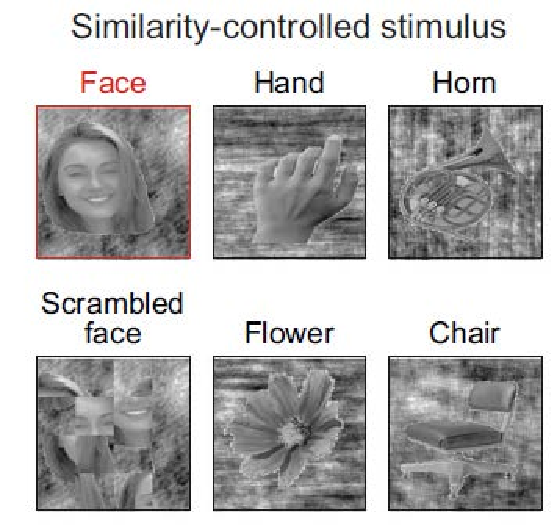
\includegraphics[width=1.0\textwidth]{figs/fig_1_c.pdf}
		\end{minipage}%
	}%
%	\subfigure[With STURE]{
%		\begin{minipage}[t]{0.48\linewidth}
%			\centering
%			\includegraphics[width=1\textwidth]{tsne_best.eps}
%		\end{minipage}%
%	}%
	%\n is important,(or \quad) 
	
	\subfigure%[Tracking results without STURE]
	{
		\begin{minipage}[t]{1.0\linewidth}
			\centering
			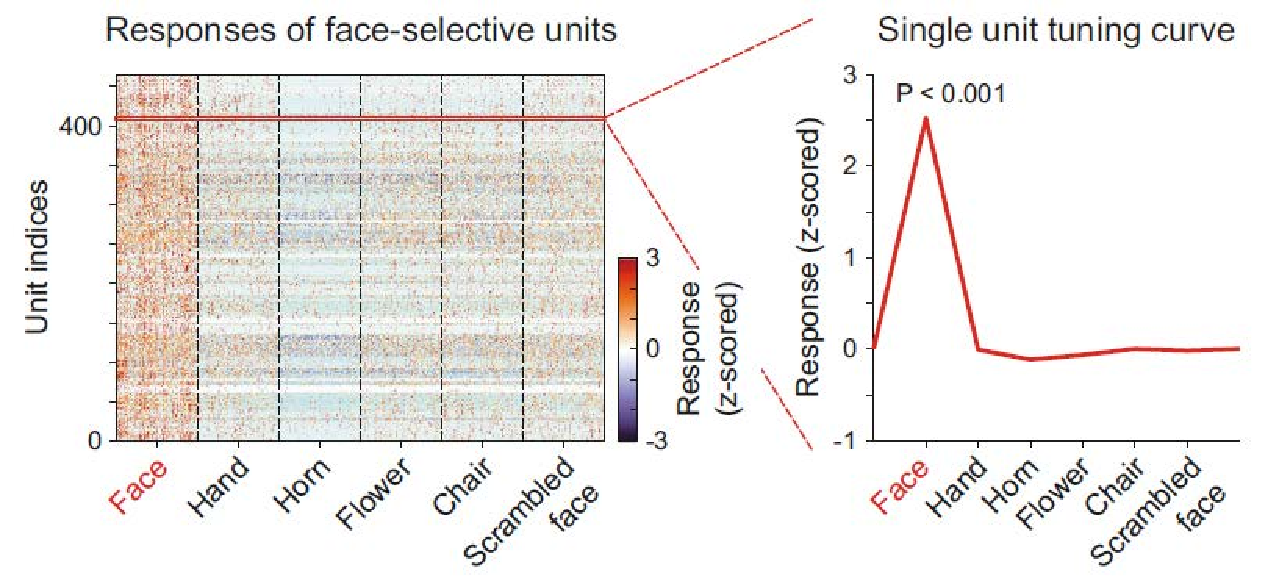
\includegraphics[width=1.0\textwidth]{figs/fig_1_d.pdf}
		\end{minipage}
	}%
%	\subfigure[Tracking results with STURE]{
%		\begin{minipage}[t]{0.48\linewidth}
%			\centering
%			\includegraphics[width=1\textwidth]{tsne_tracking_result_with_STURE.eps}
%		\end{minipage}
%	}%

	\subfigure%[Tracking results without STURE]
	{
		\begin{minipage}[t]{1.0\linewidth}
			\centering
			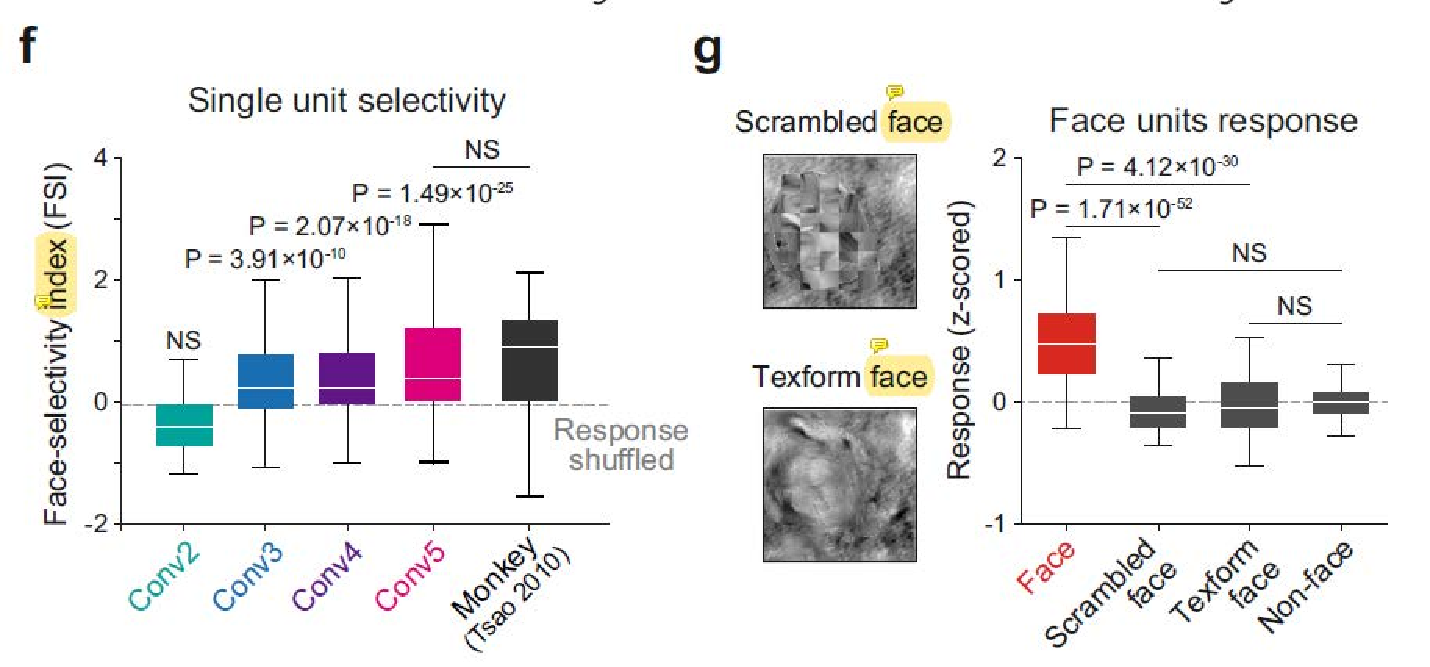
\includegraphics[width=1.0\textwidth]{figs/fig_1_f_g.pdf}
		\end{minipage}
	}
	
	\centering
	\caption{
		\textbf{Spontaneous emergence of face-selectivity in untrained networks.
		}
	\textbf{(a)} Face-select neurons and their response observed in monkey experiments.
	The response was normalized to the maximum value as 1.
	The face image shown is not the original stimulus set due to copyright.
	The image shown is available at \url{https://www.shutterstock.com} (see Methods for details).
	\textbf{(b)} the architecture of the untrained AlexNet~\cite{krizhevsky2012imagenet}.
	The untrained AlexNet was devised using a random initialization method~\cite{lecun2012efficient}, for which the values in each weight kernel were randomly sampled from a Gaussian distribution.
	\textbf{(c)} A stimulus set was designed to control the degree of intra-class image similarity.
	Stimulus images were selected and modified from a publicly available dataset that has been used in human fMRI study~\cite{stigliani2015temporal}.
	The original images are available at [\url{http://vpnl.stanford.edu/fLoc/}].
	\textbf{(d)} Responses of individual face-selective units in the untrained AlexNet ($ P < 0.001 $, two-sided rank-sum test, uncorrected).
	\textbf{(e)} The number of face-selective units in each convolutional layer in untrained networks ($ n=100 $).
	% 面部选择单元的面部选择指数
	\textbf{(f)} Face-selectivity index (FSI) of face-selective neurons in the primate IT~\cite{freiwald2010functional} ($ n=158 $), and face units in each convolutional layer in the untrained AlexNet.
	The control FSI was measured according to the shuffled responses of face-selective units in the untrained network.
	% 和打乱的人脸响应进行对比
	\textbf{(g)} (Left) Examples of texform and scrambled face images.
	(Right) Responses of face-selective units to the original face ($ n = 200 $), the scrambled face ($ n=200 $) and texform face images ($ n = 100 $).
	\textbf{(h)} Responses of face-selective units to four different sets of novel face images: 
	(1) 50 face images from our original dataset (images not used for finding face-selective units),
	(2) 16 images used in Tsao et al.~\cite{tsao2006cortical,freiwald2010functional},
	(3) 50 images used in Cao et al.~\cite{cao2018vggface2} in color and gray scale,
	and (4) 50 face images artificially generated by the FaceGen simulator (singular inversions) in color and gray scale. % Singular Inversions (软件公司)
	\textbf{(i)} The number of face-selective units, where the weight variation was changed from 5 to 200\% of the original value using two different initialization methods with Gaussian (red) and a uniform distribution (blue).
	\textbf{(j)} FSI of face-selective units across changes in the weight.
	Dashed lines indicate the mean and shaded areas indicate the standard deviation of 30 random networks.
	% 针对所有图进行说明
	All box plots indicate the inter-quartile range (IQR between Q1 and Q3) of the dataset,
	% 第三四分位数与第一四分位数的差距又称四分位距(InterQuartile Range, IQR)
	the horizontal line depicts the median and the whiskers correspond to the rest of the distribution (Q1-1.5*IQR, Q3+1.5*IQR).
	}
	\label{fig:emergence}
\end{figure*}


% 原论文主要说明发现的现象
\section{Results} 

\subsection{The emergence of face-selectivity in untrained DNNs}\par
To simulate the emergence of face-selective neurons (\Cref{fig:emergence}a), we measured the responses of a biologically inspired DNN model, AlexNet~\cite{krizhevsky2012imagenet} (\Cref{fig:emergence}b), to similarity-controlled face stimulus set (\Cref{fig:emergence}c).
A standard AlexNet model is composed of five convolutional layers (feature extraction network) and three fully connected layers (classification network), which together reproduce the structure of the ventral stream of the visual pathway (\Cref{sec:nn}).
To investigate the selective response of individual units rather than the performance of a trained system, 
we discard the classification layers and examined activity in the final layer (\Cref{fig:emergence}b,top,Conv5) of the feature extraction network.
To examine whether face tuning of units can arise even in completely untrained DNNs, 
we devised an untrained AlexNet by randomly initializing the weights of filters in each convolutional layer (\Cref{fig:emergence}b, bottom).
% 控制输入信号的长度?
For this, we used a standardized network initialization method~\cite{lecun2012efficient}, by which the weights of kernels in each convolutional layer were randomly drawn from a Gaussian distribution with parameters set to control the strength of the input signals across layers.
The stimulus set consisted of grayscale images in six different categories (\Cref{fig:emergence}c), specifically the face, a scrambled face, and four non-face objects, as previously done in monkey experiments~\cite{stigliani2015temporal}.
The images in each class were designed to control the low-level features of the luminance, contrast, object size, and object location, and they have statistically comparable intra- and inter-class image levels of similarity.


% 观察到的现象
Surprisingly, we observed a group of face-selective units ($ n = 250 \pm 63 $ in 100 random networks, mean $ \pm $ s.d.) that show significantly higher response to face images than to non-face images emerging in the untrained networks (\Cref{fig:emergence}d, $ P<0.001 $, two-sided rank-sum test).
Here, a unit is defined as a unit component at each position of the channel in an activation map of the network.
For example, there are 43,264 units (=13$\times$13$\times$256, $ N_{x-position} \times N_{y-position} \times N_{channel} $) in Conv5.
We considered each unit (of the same filter) at different spatial locations as different ones, as the selectivity of units at different locations appears to be distinct despite the fact that they share the same filter.
We also investigated the layer-specific emergence of face-selective units in untrained networks.
We found that face-selective units are also observed in earlier layers, Conv3 to 5 but are scarcely found in Conv1 and 2 (\Cref{fig:emergence}e, 
Conv1: $ n=0.008 \pm0.002\% $, 
Conv2: $ n=0.047 \pm 0.009\% $, 
Conv3: $ n=0.491 \pm 0.089\% $, 
Conv4: $ n=0.534 \pm 0.103\% $,
Conv5: $ n=0.579 \pm 0.146\% $).
We found that the number of face-selective units and the face-selectivity index (FSI) of each unit increased through the layer hierarchy (\Cref{fig:emergence}e,f).
Notably, the number of face-selective units did not show significant differences across the convolutional group or filters within each layer.
This suggests that face-selective units are not dominantly generated by a particular filter.
The number of observed face-selective units was highest in the mid- and high-level layers, similar to observations in the ventral visual pathway of monkeys~\cite{tsao2006cortical,livingstone2017development}.
These results suggest that the development of face-selectivity requires a hierarchical structure of the network along with random feedforward weights, which enables multiple linear-nonlinear computations.
We also found that the observed face-selective units in the untrained networks (Conv5) show a value of the averaged FSI~\cite{tsao2006cortical,freiwald2010functional} comparable to the index associated with monkey IT neurons (\Cref{fig:emergence}f, $ n_{untrained} = 465 $, $ n_{monkey} = 158 $, NS, two-sided rank-sum test, $ P=7.69 \times 10 ^{-2} $, $ r_{rbc} = 9.25 \times 10^{-2} $, two-sided Kolmogorov-Smirnov test, $ P=2.49 \times 10^{-4}, d=2.32 \times 10^{-2} $)
and a significantly higher value that those measured from a shuffled response (\Cref{fig:emergence}f, $ n_{untrained} = 465 $, $ n_{shuffled} = 465 $, two-sided rank-sum test, $ P=1.49 \times 10^{-25}, r_{rbc} = 5.09 \times 10^{-1} $) for various definitions of the FSI~\cite{tsao2006cortical,aparicio2016neurophysiological,duyck2021color}.
These results suggest that face-selective units, highly tuned to the face as observed in the brain, can emerge in DNNs even in the complete absence of learning.


One possible scenario for the emergence of such face-selectivity in random networks is that the observed face-selective units are simply sensitive for local face parts common to facial images.
To investigate this possibility, we measured the responses of the face-selective units to a local feature of the face using two types of control images in which global face features are disrupted but local face features are preserved.
These were (1) scrambled faces, in which small patches of the local face components were spatially scrambled, and (2) texform face~\cite{long2018mid}, in which global face features are disrupted but the statistics of the local face texture is preserved (\Cref{fig:emergence}g,left).
We confirmed that face-selective units show significantly higher responses to the original face images compared to the corresponding control images (\Cref{fig:emergence}g, right; 
Face vs. Scrambled face, $ n=200 $, one-side rank-sum test, $ P=1.71 \times 10^{-52} $, $ r_{rbc}=7.69 \times 10^{-1} $;
Face vs. Texform face, $ n=100 $, one-sided rank-sum test, $ P=4.12\times10^{-30} $, $ r_{rbc}=6.56\times 10^{-1} $).
In addition, the responses of face units to these control images were not greater than those to other non-face images, implying that face-selective units are selective to the global context of faces instead of the local components (\Cref{fig:emergence}g, right; Scrambled face vs. Non-face, $ n=200 $, one-sided Kolmogorov-Smirnov test, $ P=8.31 \times 10^{-1} $, $ d=3.00 \times 10^{-3} $; 
Texform face vs. Non-face, $ n=100 $, one-sided rank-sum test, NS, $ P=9.40 \times 10^{-1} $, $ r_{rbc}=4.51 \times 10^{-2} $, $ d=1.84 \times 10^{-2} $).
These results suggest that the observed face units in the untrained network are not particularly selective to local face parts, but are instead selective to a whole face.


% h
Next, we investigated the responses of face-selective units to four different novel stimulus sets that were not used to find face-selective units.
These were
(1) 50 face images from our original data set, not used for finding the face-selective units;
(2) 15 face image used in Tsao et al.~\cite{tsao2006cortical,freiwald2010functional};
(3) 50 face images used in Cao et al.~\cite{cao2018vggface2};
and (4) 50 face images artificially generated by the FaceGen simulator (singular inversions) in color and grayscale (\Cref{fig:emergence}h).
We found that face-selective units in the untrained network show significantly higher responses to novel face images compared to the responses to non-face under all conditions (\Cref{fig:emergence}h, Novel face vs. Non-face images, one-sided rank-sum test, $ P \leq 1.47 \times 10^{-11} $, $ r_{rbc} \geq 4.54 \times 10^{-1}$).
These results suggests that the observed face-selectivity in an untrained network defined by one specific dataset can be generalized to other novel sets of faces.


% figure i, j
To confirm that the emergence of face-selective units is not due to the specific initial parameter set but is rather generally observed in an untrained network,
we varied the width of the weight distribution for random network initialization (Gaussian and uniform) from 5 to 200\% of the original standard deviation of the standardized random initialization and examined if face-selective units consistently emerge (\Cref{fig:emergence}i,j).
We found that face-selective units consistently arise in the untrained networks across the variation of the parameter.
The number (\Cref{fig:emergence}i) and selectivity index (\Cref{fig:emergence}j) of observed face units were largely unchanged across a wide range of weight variations and across the wide variation in the width of the weight distribution.
This implies that the emergence of face-selective units in untrained networks is highly robust to variations of the wiring strength.


\begin{figure*}[htbp]
	\centering
	
	\subfigure%[Without STURE]
	{
		\begin{minipage}[t]{0.8\linewidth}
			\centering
			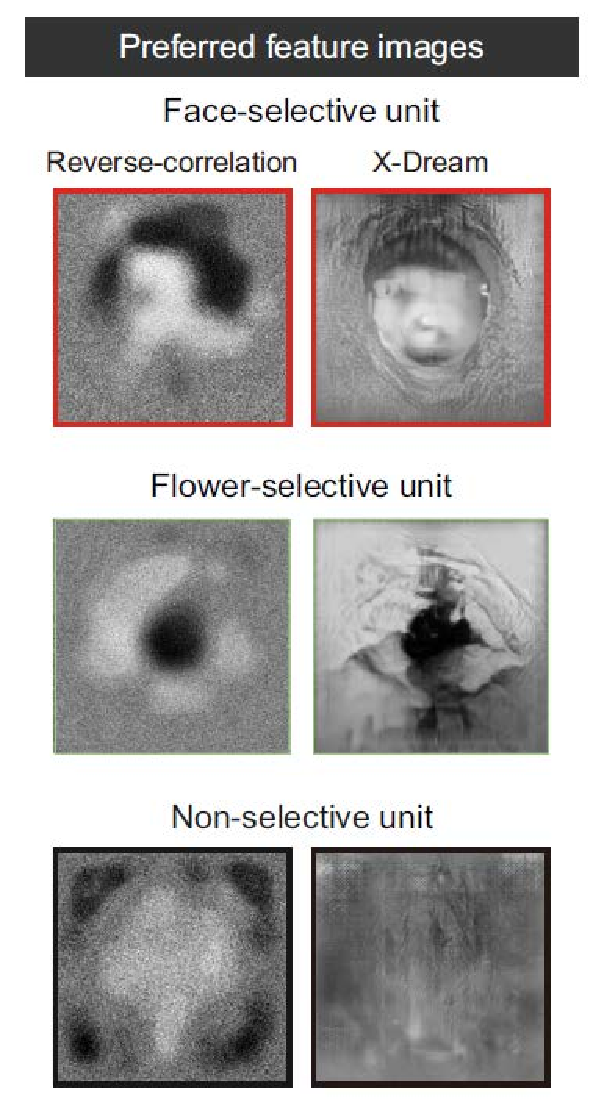
\includegraphics[width=1.0\textwidth]{figs/fig_2_c.pdf}
		\end{minipage}%
	}%
	
	
	\centering
	\caption{
		\textbf{Preferred feature images of face-selective units in untrained networks.
		}
		\textbf{(a)} Measurements of preferred feature images (PFI) of target units in Conv5 from the reverse-correlation analysis~\cite{bonin2011local}.
		Bright and dark 2D Gaussian filters were generated at a random position as an input stimulus set.
		The PFI was obtained as the summation of stimuli weighted by the corresponding response.
		The initial preferred feature image was calculated from the local Gaussian stimulus set by the classical reverse-correlation method~\cite{bonin2011local}.
		% RNN?
		Then, a new stimulus set was generated as the summation of the obtained PFI and local Gaussian stimuli, with the second preferred feature image then obtained from a new stimulus set.
		This procedure was repeated to obtain the preferred feature image.
		\textbf{(b)} Schematics of the process used to achieve a preferred feature image (PFI) using a generative neural network (GAN) and a genetic algorithm (X-Dream)~\cite{ponce2019evolving}.
		Synthesized images are generated by the GAN with image codes and are fed into an untrained network as input.
		The genetic algorithm finds a new image code that maximizes the response of the target unit.
		The PFI of a target unit is achieved after 100 iterations of this procedure.
		\textbf{(c)} The obtained preferred feature images, using the reverse-correlation method and X-Dream, of the face-selective unit, selective units to non-face class (flower), and units selective to none of the class.
		\textbf{(d)} Illustration of the face-configuration index (FCI) of a face unit's PFI.
		The FCI was defined as pixel-wise correlation between the original face stimuli and the generated PFIs.
		\textbf{(e)} FCI of PFI, using the reverse correlation method, of units selective to each class ($ n_\textrm{Face} = 465 $, $ n_\textrm{Hand} = 7 $, $ n_\textrm{Horn} = 772 $, $ n_\textrm{Flower} = 107 $, $ n_\textrm{Chair} = 63 $).
		\textbf{(f)} FCI of PFI, using X-Dream, of the same units as the units used in (\textbf{e}).
		All box plots indicate the inter-quartile range (IQR between Q1 and Q3) of the dataset,
		the horizontal line depicts the median and the whiskers correspond to the rest of the distribution (Q1-1.5*IQR, Q3+1.5*IQR).
		The face images shown in panels (\textbf{d})-(\textbf{f}) are selected examples from the publicly available dataset~\cite{stigliani2015temporal}.
		The original images are available at [\url{http://vpnl.stanford.edu/fLoc}].
	}
	\label{fig:preferred}
\end{figure*}

\subsection{Preferred feature images of face-selective units in an untrained network}

Next, to characterize the feature-selective responses of these face-selective units qualitatively,
we reconstructed preferred feature images (PFI) of individual units using a reverse-correlation (RC) method~\cite{bonin2011local} and a generative adversarial network algorithm (X-Dream)~\cite{ponce2019evolving} (see~\Cref{sec:preferred}).
In the RC analysis, we presented 2500 images of bright and dard 2D Gaussian filters at random positions as input stimuli to an untrained network (\Cref{fig:preferred}).
By adding stimuli weighted according to the corresponding neural response with 100 repeated iterations, we obtained the preferred feature images of the target units.
In the X-Dream analysis, a deep generative adversarial neural network~\cite{dosovitskiy2016generating} was trained to ImageNet datasets to synthesize preferred feature images from the image codes scored by a genetic algorithm using the responses of units from repeated iterations. (\Cref{fig:preferred}b).
We found that the response of target units induced by the PFI was increased, being higher that those induced by face stimulus images, as the iteration number of the genetic algorithm exceeds a certain value 
(\Cref{fig:preferred}a, right, $ n=465 $, 
RC PFI vs. face stimulus, two-sided rank-sum test, $ P=1.51 \times 10^{-6} $, $ r_{rbc} = 1.58 \times 10^{-1} $;
RC PFI vs. non-face stimulus, two-sided rank-sum test, $ P=3.12 \times 10^{-2} $, $ r_{rbc} = 7.07 \times 10^{-2} $,
\Cref{fig:preferred}b, right, $ n=465 $, 
X-Dream PFI vs. face stimulus, two-sided rank-sum test, $ P=1.92 \times 10^{-119} $, $ r_{rbc} = 7.63 \times 10^{-1} $;
X-Dream PFI vs. non-face stimulus, two-sided rank-sum test, $ P = 2.68 \times 10^{-129} $, $ r_{rbc} = 7.94 \times 10^{-1} $
).
These results indicate that our PFI generation methods successfully find the most preferred input feature of face-selective units.
As a result, using both methods, we obtained the PFI of face-selective units, units selective to non-face classes, and units without selective responses to any image classes (\Cref{fig:preferred}c).
We found that the PFI of the face-selective units presents distinguishable features from those of other objects.
We observed that the PFIs of face-selective units represent face-like configurations, whereas the PFIs of units selective to non-face classes show noticeable configurations of each object class (i.e., flowers in an RC and X-Dream).


% d
To quantify the structural similarity of the PFIs to face images, we defined the face-configuration index as the averaged pixel-wise correlation between a PFI and the 200 face images used for face unit selection (\Cref{fig:preferred}d).
We estimated the face-configuration index of each PFI of face-selective and non-face-selective units generated by the RC method.
We found that the estimated PFIs of face-selective units (with a visually observable face-like configuration) have a significantly higher average value of the index than that from the units selective to non-face objects (\Cref{fig:preferred}e, 
Face PFI vs. Non-face PFI, 
$ n_\textrm{Face}    = 465 $,
$ n_\textrm{Horn}    = 772 $,
$ n_\textrm{Hand}    = 7   $,
$ n_\textrm{Chair}   = 63  $,
$ n_\textrm{Flower}  = 107 $,
one-sided rank-sum test,
$ P \leq 5.63 \times 10^{-4} $,
$ r_{rbc} \geq 1.56 \times 10^{-1} $;
\Cref{fig:preferred}f, Face PFI vs. Non-face PFI,
$ n_\textrm{Face}   = 465 $,
$ n_\textrm{Chair}  = 63  $,
$ n_\textrm{Horn}	= 773 $,
$ n_\textrm{Hand}	= 7	  $,
$ n_\textrm{Flower}	= 107 $,
one-sided rank-sum test, 
$ P \leq 1.93 \times 10^{-5} $,
$ r_{rbc} \geq 2.35 \times 10^{-1} $
).
Notably, the average pairwise correlation estimated between each face stimulus image shows a significantly lower value of nearly zero, 
implying that the observed index of face-selective units reflects structural similarity to the averaged (or a prototype, abstract) face image rather than similarly to particular face images accidentally observable.


Next, we hypothesized that the observed face-selective units may encode invariant representations of the prototype face images, as some types of intrinsic are a basic property of CNNs.
A number of previous studies suggested that various types of invariance (e.g., translation, scaling, and rotation) over a wide range of image transformations can be implemented in a CNN~\cite{lecun2004learning,kavukcuoglu2010learning,lecun2012learning,chidester2018rotation,srivastava2018effect}, mostly due to three key components--the convolutional layer, the pooling layer, and the hierarchical structure--in CNN models.
Thus, to investigate whether the observed face-selective units show invariant representations of face images regardless of corresponding image condition, 
we measured the response of face-selective units to face and non-face object images with various positions, sizes, and rotation angles.
First, we observed that single face units show constant face tuning under a fairly wide range of size/potion/rotation variations and that range was comparable with those of face-selective neurons in IT~\cite{zoccolan2007trade}.
Notably, we found that our model units also show the inversion effect observed in monkeys~\cite{tsao2006cortical,buiatti2019cortical,perrett1985visual}.
We found that the response of face-selective units to inverted face images are significantly lower that those to upright faces.


Similarly, we found viewpoint-invariant face-selective units and mirror-symmetric viewpoint-specific units in a random network.
Interestingly, the number of viewpoint-invariant face-selective units increased along the network hierarchy, similar to previous observations in the brain~\cite{freiwald2010functional}.
These results show that the observed invariances can arise from the hierarchical structure with convolutional filtering without the contribution of structured spatial filters.
Notably, the current result also suggests a possible scenario through which to understand how viewpoint invariant selectivity can arise in infant animals.
From the similarities between the CNN and the biological brain models, i.e., that the fundamentals of both CNNs and sensory cortices are based on the hierarchical feedforward structure and that the process of convolution via weight sharing in CNNs can be approximated by a biological model of periodic functional maps with hypercolumns in the visual cortex,
our result may inspire insight into how innate invariance can arise in infant animals.



\begin{figure*}[htbp]
	\centering
	
	\subfigure%[Without STURE]
	{
		\begin{minipage}[t]{1.0\linewidth}
			\centering
			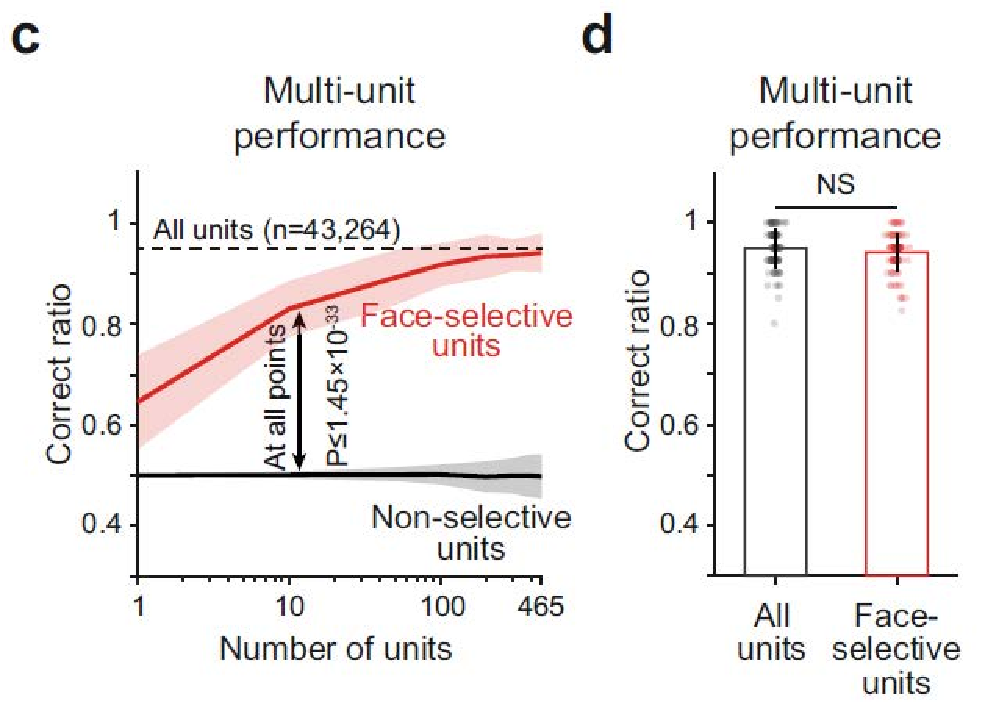
\includegraphics[width=1.0\textwidth]{figs/fig_3_c_d.pdf}
		\end{minipage}%
	}%
	
	
	\centering
	\caption{
		\textbf{Detection of face images using the response of face units in untrained networks.
		}
	(\textbf{a}) Design of the face detection task and SVM classifier using the responses of the untrained AlexNet.
	During this task, face or non-face images were randomly presented to the networks and the observed response of the final layer was use d to train a support vector machine (SVM) to classify whether the given image was a face or not.
	Among 60 images from each class (face, hand, horn, flower, chair, and scrambled face) that were not used for face unit selection, 40 images were randomly sampled for the training of the SVM, and the other 20 images were used for testing.
	The images shown are selected examples from the publicly available dataset~\cite{stigliani2015temporal}.
	The original images are available at [\url{http://vpnl.standford.edu/fLoc}].
	(\textbf{b}) Performance on the face detection task using a single unit randomly sampled from face-selective units ($ n = 465 $) and units without selective responses to any image classes ($ n = 7776 $).
	The channel level was measured by the shuffled responses of face-selective units in the untrained network.
	The error bar indicates the standard deviation of each unit.
	Each bar indicates the mean and the error bar indicates the standard deviation of performance of each unit.
	(\textbf{c}) Performance of the face detection task using face-selective units and non-selective units when varying the number of units from 1 to 456.
	The dashed line indicates the detection performance using all units in Conv5 ($ n=43,264 $).
	Each line indicates the mean and the shaded area indicates the standard deviation for 100 repeated trials of the random sampling of units.
	(\textbf{d}) Performance on the face detection task using face-selective units ($ n=465 $) and then using all units in Conv5 ($ n=43,264 $).
	Each bar indicates the mean and the error bar indicates the standard deviation for 100 repeated trials of the random sampling of units.
	}
	\label{fig:detection}
\end{figure*}

\subsection{Detection of face images using the responses of face-selective units}
We tested whether the selective responses of these face units could provide reliable information with which to detect between faces and non-face objects.
During this task, face ($ n=40 $) or non-face ($ n=40 $) images were randomly presented to the networks, and the observed response of the final layer was used to train a support vector machine (SVM) to classify whether the given image was a face or not (\Cref{fig:detection}a).
First, we compared the detection performance of the SVM using a single unit randomly sampled from face-selective units and using units without selective responses to any image classes.
We confirmed that the SVM trained with a single face-selective unit shows noticeably higher performance that those measured from shuffled responses, whereas the SVM trained with units without selectivity does not 
(\Cref{fig:recognition}b,
Face unit vs. Response shuffled, 
$ n_\textrm{face} = 465 $,
two-sided rank-sum test,
$ P = 2.97 \times 10 ^{-121} $,
$ r_{rbc} = 7.68 \times 10^{-1} $;
Response shuffled vs. Non-selective unit, 
$ n_\textrm{non-selective} = 7,776 $,
two-sided rank-sum test, NS, 
$ P = 1.10 \times 10^{-1} $,
$ r_{rbc} = 4.52 \times 10^{-2} $,
two-sided Kolmogorov-Smirnov test,
$ P = 1.93 \times 10^{-1} $,
$ d = 2.12 \times 10^{-2} $
).
Then, extending the test to various numbers of units, we compared the detection performance of this SVM using face-selective units with the performance when using the same number of randomly sampled non-selective units.
We confirmed that the SVM trained with multiple face-selective units shows noticeably better performance that that trained with the same number of non-selective units, 
as the number of units used in each condition was varied from $ n=1 $ to 465 (total number of face units in untrained networks)
(\Cref{fig:recognition}c,
Face vs. Non-selective units, 
$ n_\textrm{trial} = 100 $,
two-sided rank-sum test, 
$ P \leq 1.45 \times 10^{-33} $,
$ r_{rbc} \geq 8.74 \times 10^{-1} $
).
We also found that the SVM using face units ($ n=465 $) nearly matches the performance of the SVM using all units in the final layer ($ n=43,264 $)
(\Cref{fig:recognition}d, 
Face vs. All units, 
$ n_\textrm{trial} = 100 $,
two-sided rank-sum test, NS, 
$ P = 1.90 \times 10^{-1} $,
$ r_{rbc} = 9.29 \times 10^{-2} $,
two-sided Kolmogorov-Smirnov test,
$ P = 1.90 \times 10^{-1} $,
$ d = 9.20 \times 10^{-3} $
).
Furthermore, we found that face units enable the networks to detect faces with various sizes, position, and rotations even when such image conditions were held constant when training the SVM classifier.


Notably, we also found that the SVM can successfully detect faces when it is trained with the responses of units selective to non-face classes, 
similar to the results in a previous experiment in human~\cite{haxby2001distributed},
whereas it failed to detect with units not selective to any of the classes.
To compare our results with the experiment condition of the previous human experiment~\cite{haxby2001distributed},
we first trained the SVM using the responses of four distinct populations:
(1) all of the units selective to each class (All-selective),
(2) units selective to non-face classes (Non-face-selective),
(3) face-selective units only (Face-selective),
and (4) units not selective to any of the classes (Non-selective).
As a result, we found that the SVM trained with non-face-selective units showed a performance comparable with the results of Haxby et al.~\cite{haxby2001distributed}.
Interestingly, the performance was also comparable with those with all-selective units and those with face-selective units only,
similar to the results in a previous experiment in human~\cite{haxby2001distributed}.
This result is understandable considering that there are only five image classes;
thus, even non-face-selective units can provide information for discriminating face and non-face images by generating different levels of activities for each class.
Taken together, these results imply that the information provided by selective units that emerge in the untrained networks is sufficient to detect between faces and non-face objects.


\begin{figure*}[htbp]
	\centering
	
	\subfigure%[Without STURE]
	{
		\begin{minipage}[t]{1.0\linewidth}
			\centering
			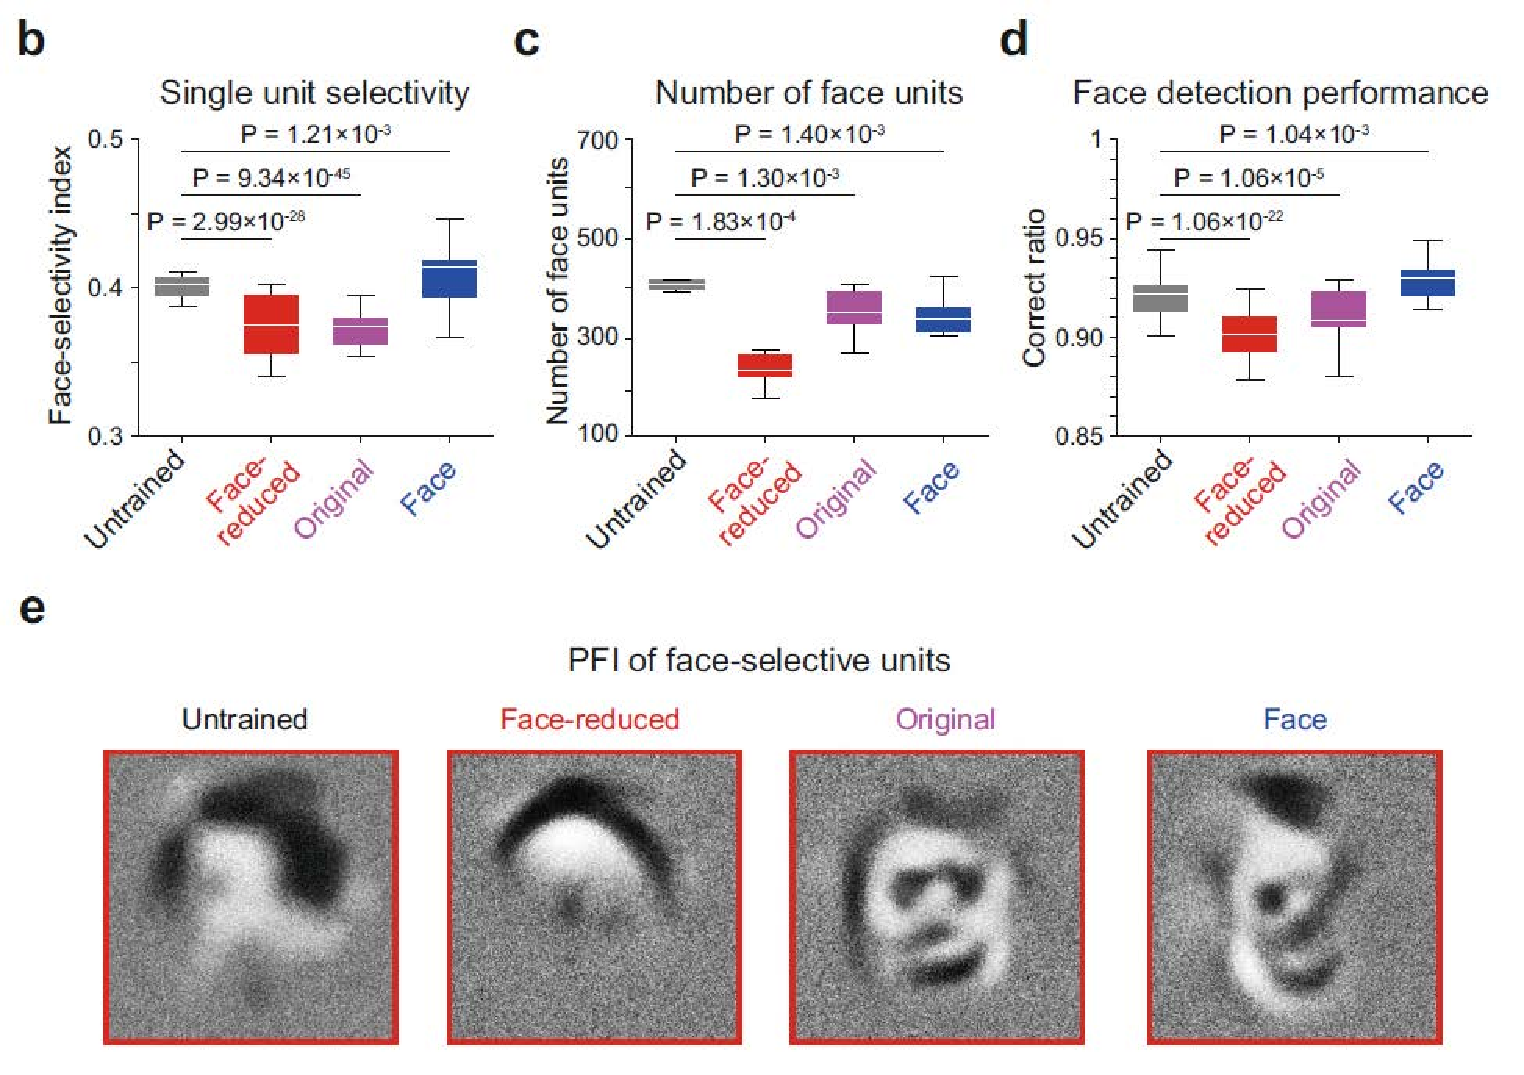
\includegraphics[width=1.0\textwidth]{figs/fig_4_b_f.pdf}
		\end{minipage}%
	}%
	
	
	\centering
	\caption{
		\textbf{Effect of training on face-selectivity in untrained networks.
		}
	(\textbf{a}) Three different datasets modified from publicly available ImageNet~\cite{ILSVRC15} were used for the training of the network for image classification: 
	(1) face-reduced ImageNet, 
	(2) original Imagenet, 
	and (3) ImageNet with added face images.
	For copyright reasons, the face image shown here is not the actual image used in the experiments.
	The original images are replaced with images with similar contents for display purposes.
	The original images are available at [\url{https://www.image-net.org/download}].
	Images shown are available at [\url{https://www.shutterstock.com},\url{http://vpnl.stanford.edu/fLoc/}~\cite{stigliani2015temporal}].
	(\textbf{b}) Face-selectivity index of face-selective units in untrained network and in networks trained with the three datasets ($ n_\textrm{Untrained} = 4,267 $, $ n_\textrm{Reduced} = 2,452 $, $ n_\textrm{Original} = 3,561 $, $ n_\textrm{Face} = 3,585 $).
	(\textbf{c}) The number of face-selective units in untrained networks and in networks trained with three datasets ($ n_\text{net} = 10 $).
	(\textbf{d}) Face detection performance of untrained networks and of networks trained with three different datasets ($ n_\textrm{trial} = 1,000 $).
	(\textbf{e}) The obtained preferred feature images (PFI), using reverse-correlation method of the face-selective unit on each network.
	All box plots indicate the inter-quartile range (IQR between Q1 and Q3) of the dataset,
	the horizontal line depicts the median and the whiskers correspond to the rest of the distribution (Q1-1.5*IQR, Q3+1.5*IQR).
	}
	\label{fig:effect}
\end{figure*}

\subsection{The emergence of face-selectivity in trained DNNs}
We tested a scenario in which our current model can corroborate the conflicting observations regarding the role of visual experience for the development of face-selectivity.
A previous report suggested that visual experience is necessary for the emergence of face-selectivity by showing that monkeys raised without exposure to faces lack face-selective domains~\cite{arcaro2017seeing}.
On the other hand, another recent study showed that the face-selective area develops robustly in congenitally blind humans, suggesting that visual experience is not necessary for face-selectivity~\cite{arcaro2017seeing}.
Regarding these conflicting results, we examined how face-selective units in untrained networks can be affected by training with visual inputs.


To investigate the effect of training on a face image set,
we prepared the following three different stimulus sets:
(1) face-reduced ImageNet: 500 classes including no recognizable face images were manually curated from the ILSVRC 2010 dataset according to a visual inspection by the authors,
(2) the original ImageNet, 
and (3) the original ImageNet with added face images used in the current study~\Cref{fig:effect}a.
Then, the network was trained with each of these image sets.
First, we found that the FSI of the face-selective units was significantly decreased after being trained to the face-reduced image set 
(~\Cref{fig:effect}b,
Untrained vs. Face-reduced,
$ n_\textrm{Untrained} = 4,267 $,
$ n_\textrm{Reduced} = 2,452 $,
two-sided rank-sum test,
$ P = 2.99 \times 10^{-28} $,
$ r_\textrm{rbc} = 6.76 \times 10^{-1} $
),
whereas it was increased after being trained to the face-including image sets 
(Untrained vs. Face-included,
$ n_\textrm{Face} =3585 $,
two-sided rank-sum test,
$ P = 1.21 \times 10^{-3} $,
$ r_{rbc} = 2.60 \times 10^{-1} $
).
Notable, the FSI was significantly decreased after being trained to the original ImageNet dataset that contains images of faces but has no group labeled as face
(~\Cref{fig:effect}b, Untrained vs. Original, 
$ n_\textrm{Original} = 3,561 $,
two-sided rank-sum test,
$ P = 9.34 \times 10^{-45} $,
$ r_\textrm{rbc} = 8.15 \times 10^{-1} $
).
This suggests that the tuning of face-selective units could either be sharpened or weakened by training with distinct stimulus sets.

% Fig.4 c
Next, we found that the number of face-selective units observed was greater in the network trained with face-including image set compared to that trained to face-reduced images 
(~\Cref{fig:effect}c, Untrained vs. Trained,
$ n_\textrm{Net} = 10 $,
two-sided rank-sum test,
$ P \leq 1.40 \times 10 ^{-3} $,
$ r_\textrm{rbc} \geq 5.72 \times 10^{-1} $
).
Interesting, however, we found that the number of face-selective units, when trained to face-including images, appeared to be smaller than that of untrained networks.
These results imply that the training process of the network to face-including images selectively sharpens the tuning of face units so that the selectivity of strongly tuned units is sharpened while the weakly tuned units are pruned.
In this condition, the face detection performance of the networks would improve in face-trained networks even if the number of face units decreased compared to the initial, untrained condition.
To validate this scenario, we trained the SVM using the response of face-selective units for a face detection task in an untrained network and in the three networks trained to each type of data set.
As predicted, we found that the face detection performance was significantly increased in the networks trained to the face-including image set compared to that of the untrained network
(~\Cref{fig:effect}d, Untrained vs. Face included, 
$ n_\textrm{trial} = 1000 $,
two-sided rank-sum test,
$ P = 1.04 \times 10^{-3} $,
$ r_\textrm{rbc} = 2.60 \times 10^{-1} $
),
whereas the face detection performance of the network trained to the face-reduced image set was significantly decreased compared to the untrained network
(~\Cref{fig:effect}, Untrained vs. Face-reduced,
$ n_\textrm{trial} = 1,000 $,
two-sided rank-sum test,
$ P = 1.06 \times 10^{-22} $,
$ r_\textrm{rbc} = 6.42 \times 10^{-1} $
).
Furthermore, we found that the PFI of the face-selective unit shows a clear face configuration in the network trained to face-including natural images,
whereas the face configuration is disrupted in network trained to face-reduced dataset (~\Cref{fig:effect}e).
This result is consistent with previous observation of decreased face-selectivity in face-deprived monkeys~\cite{arcaro2017seeing}.



\begin{figure*}[htbp]
	\centering
	
	\subfigure%[Without STURE]
	{
		\begin{minipage}[t]{1.0\linewidth}
			\centering
			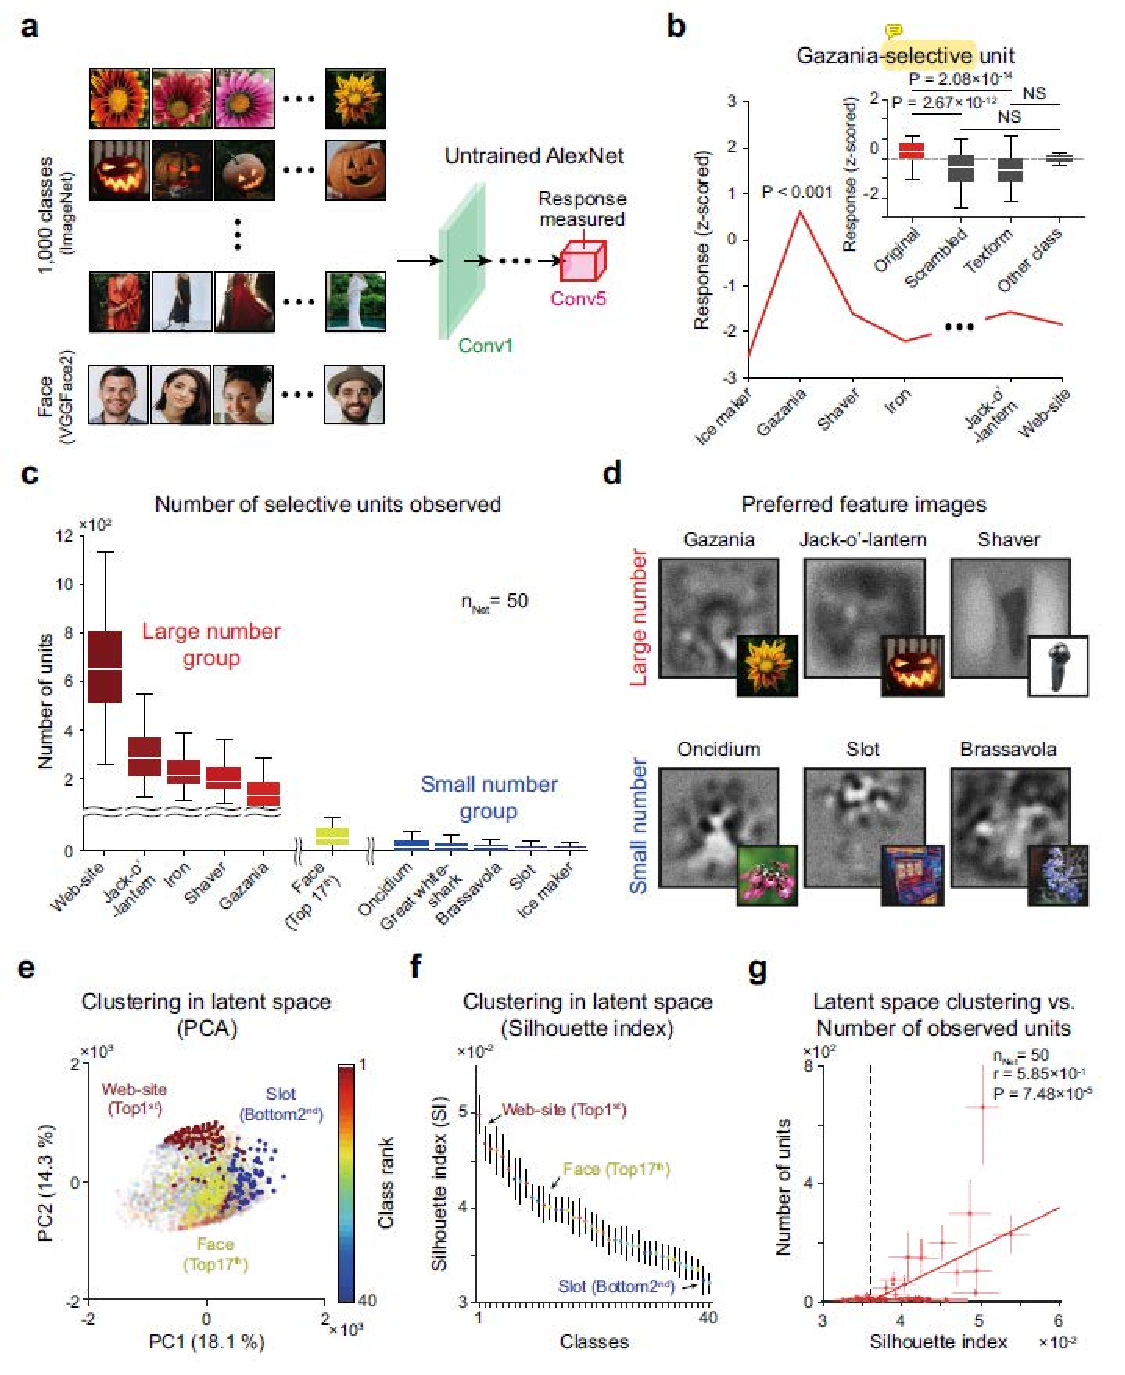
\includegraphics[width=1.0\textwidth]{figs/fig_5_a-f_1.pdf}
		\end{minipage}%
	}%
	
	\centering
	\caption{
		\textbf{ImageNet category-selective units in untrained networks.
		}
	(\textbf{a}) The responses of units in untrained networks to the images of 1,000 ImageNet~\cite{ILSVRC15} classes and to face images (VGGFace2)~\cite{cao2018vggface2}.
	% 杂色菊
	(\textbf{b}) Average tuning curve of gazania selective units.
	(Inset) Responses of gazania-selective units to the original gazania ($ n = 100 $), the scrambled gazania ($ n = 100 $) and texform gazania images ($ n = 100 $).
	(\textbf{c}) The number of selective units for 39 classes in which selective units are observed.
	The error bar indicates the standard deviation of 50 random networks.
	%	
	(\textbf{d}) Sample preferred feature images achieved by reverse-correlation analysis and stimulus images (inset).
	% 
	(\textbf{e}) Visualization of the PCA (principal component analysis)~\cite{wold1987principal} analysis results (only two principal components (PC) are shown) using the Conv5 unit response to each class in untrained networks.
	The analysis was performed using 3,999 principal components, and the top $140 \pm 32$ components contained $ 75\% $ of the variance.
	% 轮廓系数(Silhouette Coefficient),是聚类效果好坏的一种评价方式。
	(\textbf{f}) The silhouette index~\cite{kaufman2009finding} of the Conv5 unit responses was measured using all principal components to estimate the consistency of data clustering.
	Each dot indicates the mean and the error bar indicates the standard deviation of 50 simulations of randomly initialized networks.
	% 
	(\textbf{g}) Correlation between the silhouette index and the number of selective units observed (Pearson correlation).
	Each dot indicates the mean and the error bar indicates the standard deviation of 50 random networks.
	%
	All box plots indicate the inter-quartile range (IQR between Q1 and Q3) of the dataset, the horizontal line depicts the median and the whiskers correspond to the rest of the distribution (Q1-1.5*IQR, Q3+1.5*IQR).
	For copyright reasons, the images in panels (\textbf{a}) and (\textbf{d}) are not the actual images used in the experiments.
	The original images are replaced with images with similar contents for display purposes.
	The original images are available at [\url{https://www.image-net.org/download}, \url{https://arxiv.org/abs/1710.08092}].
	Images shown are available at [\url{https:/www.shutterstock.com}].
	}
	\label{fig:image_net}
\end{figure*}

\subsection{The emergence of selectivity to various objects in untrained DNNs}
Lastly, we investigated the possibility that units selective to various objects other than faces also emerge similarly in untrained neural networks.
For this, we measured the responses of units in random networks to a stimulus dataset of ImageNet containing 1,000 classes of objects (~\Cref{fig:image_net}a).
As a result, we found that selective units are observed in 39 classes among the 1,000 classes (~\Cref{fig:image_net}b,c).
From the analysis using scrambled and texform control images, we confirmed that these object-selective units are not particularly selective to local image parts but are selective to a whole object, similar with units selective to faces
(~\Cref{fig:image_net}b, inset,
Gazania vs. Scrambled gazania, 
$ n=100 $,
one-sided rank-sum test,
$ P = 2.67 \times 10^{-12} $,
$ r_\textrm{rbc} = 4.89 \times 10^{-1} $,
%
Gazania vs. Texform gazania, 
$ n = 100 $,
one-sided rank-sum test, NS,
$ P = 1.00 $,
$ r_\textrm{rbc} = 3.17 \times 10^{-1} $,
one-sided Kolmogorov-Smirnov test,
$ P = 1.02 \times 10^{-2} $,
$ d = 2.97 \times 10^{-2} $;
% 
Texform gazania vs. other-class,
$ n = 100 $,
one-sided Kolmogorov-Smirnov test,
$ P = 3.45 \times 10^{-2} $,
$ d = 2.55 \times 10^{-2} $
).
This result suggests that units selective innately to various objects such as faces can emerge in untrained neural networks.


Next, to investigate the emergent condition of units selective to each object further, we sorted those 39 classes according to the number of selective units observed and computed the PFI using the RC method (~\Cref{fig:image_net}c,d).
In general, we observed a tendency in which the PFIs of the large number group showed a relatively simple configuration of each preferred object class that was visually observable (~\Cref{fig:image_net}d, top), 
whereas those of the small number classes represented a more complicated structure of the PFI (~\Cref{fig:image_net}d, bottom).
From this result, we hypothesized that objects with a simple configuration, such as faces, can induce stronger clustering in the latent space representation than those of other object classes and therefore may have a greater likelihood of generating units selective to them.
To validate our hypothesis, we used the dimension-reduction method~\cite{wold1987principal} to compare a clustered representation of each object class in terms of the raw pixel values and in the responses of Conv5.
For quantification of the representational clustering of each class, we measured the silhouette index~\cite{kaufman2009finding} to estimate the consistency of data clustering.
We found that there is a strong correlation between the silhouette index in the Conv5 latent space and the number of selective units observed
(~\Cref{fig:image_net}e-g, Pearson correlation coefficient,
$ n_\textrm{Net} = 50 $,
$ r = 5.85 \times 10^{-1} $,
$ P = 7.48 \times 10^{-5} $
).
This result demonstrates that objects with a simple profile, readily distinguishable from those of other objects statistically, lead to a strong clustering of abstracted responses in the DNN and are more likely to generate units selective to it.
Furthermore, the relationship between the silhouette index and the number of units observed shows that the number of units increases as the silhouette index increases,
with no selective units observed when the silhouette index is below 0.036 (~\Cref{fig:image_net}g, black dashed line).
This result implies that there may be a threshold of the clustering level in the response embedding space, by which a unit selective to that object class can be defined and observed.
In neuroscience, this may provide a possible explanation of why face-selective neurons are observed in various experiments while neurons selective to other objects are not observed as readily.
Thus, the observed face-selectivity may not be a special case of tuning, 
whereas selectivity to other visual objects can also arise in random networks simply due to the relatively simple configuration of the corresponding geometric components.



\section{Discussion}
We showed that a biologically inspired DNN develops face-selective units without training, solely from statistical variations of the feedforward projections.
These results suggest that the statistical complexity embedded in the structure of the hierarchical circuit~\cite{paik2011retinal,jang2017interlayer,sailamul2017synaptic} can initialize primitive cognitive functions such as face-selectivity in untrained neural networks.
Although the performance of a DNN appears to be similar to that of the brain on certain visual tasks, 
there are critical differences between biological brains and DNN models, such as convolutional filtering in DNN models, which is not biologically plausible.
However, although DNNs are not an impeccable model of the visual pathway of the brain, 
the current results provide a possible scenario for understanding how primitive visual functions such as face detection can initially arise in early brains before learning begins with sensory inputs.


State-of-the-art studies using random networks provide important clues regarding how these selective units can arise spontaneously in untrained model networks.
Recently, it was reported that a network can classify an untrained image class by combining pre-trained readout units~\cite{socher2013zero}, a process known as zero-shot learning.
Our results suggest that such zero-shot learning is even possible without any pre-trained readout units.
It was also reported that an artificial network that learns visual features with random, untrained weights can perform image classification tasks~\cite{jarrett2009best,pinto2009high}.
Jarrett et al. showed that features from a randomly initialized one-layer convolutional network could classify the Caltech 101 dataset with a performance level similar to that of fine-tuned network, 
consistent with the mathematical notion that a combined convolutional and pooling architecture could develop spatial frequency selectivity and translation invariance~\cite{saxe2011random}.
Overall, these results suggest that the initial structure of random networks plays an important role in visual feature extraction before the training process.
They also imply that complex types of feature selectivity, such as face-selectivity, may arise innately from the structure of the random feedforward circuitry.


Furthermore, recent model studies using the lottery ticket hypothesis~\cite{frankle2019stabilizing,ramanujan2020s} showed that randomly weighted neural networks contain subnetworks that can perform tasks without modifying the initial random weight values,
implying that functional architectures can emerge from random initial wirings.
This model and our current model have a common aspect in that functional structures can emerge without any modification to the initial random weights.
However, the lottery ticket hypothesis showed that a random subnetwork can perform tasks without learning,
while our model demonstrates that the functional tuning of single units can arise spontaneously.
Indeed, our model not only suggests a possible mechanism of the origin of the functional tuning of single neurons in the early developmental process in the brain but also provides insight into the mechanism underlying the emergence of functional subnetworks, 
possibly from tuned individual units that emerge in random artificial neural networks.


% 储备池计算
% RC的好处是特征提取网络,即Reservoir ,是随机生成并在训练和预测阶段是固定的,只有readout部分是要学的
Similarly, the theory of reservoir computing suggests that the circuits required for higher-order cognitive functions, such as classification, may already exist in untrained, random recurrent neural networks.
In this scenario, higher-order cognitive functions can be achieved only by training a read-out network, as suggested by the lottery ticket hypothesis~\cite{verstraeten2007experimental,bellec2020solution}.
Interestingly, our results in the face-detection task performed with the SVM are comparable to the concept of reservoir computing, 
as the training of the SVM with the responses of untrained networks is consistent with the procedure of training a read-out projection from random networks in reservoir computing.
It is notable that recent studies suggest that the random network can perform this task if the read-out units are selected via a prior understanding of the system.
For example, object classification can be performed by a random network if read-outs are chosen by a synaptic rule observed in the brain~\cite{weidel2021unsupervised,tetzlaff2013synaptic}.
While these models focus on the innate functions of networks in that a high dimensional space generated by a random network can perform various tasks without learning,
our current results demonstrate that the functional tuning of single units (comparable to neuronal tuning in biological brains) can arise in random networks without any further training of the read-out process, 
which is distinguished from the main idea of the reservoir computing model.


It is important to note that the current results do not necessarily mean that innate face-selectivity is the tuning observed in adult animals.
There is a wealth of evidence showing that higher areas of the visual cortex are immature in the early development stage and that the corresponding functional circuit is modulated by visual experience~\cite{zhang2005delayed,baldwin2012cortical,bourne2006hierarchical,kiorpes2004neural}.
There is also strong evidence that the IT region, where face-selective neurons are observed, can be altered by early experience~\cite{srihasam2012behavioral,srihasam2014novel}.
Considering the anatomical and physiological changes that occur over the first postnatal year, 
the innate template of face-selective neurons in very early developmental stages must be refined by later visual experience, including both bottom-up and top-down processes~\cite{yan2018bottom,epshtein2008image}.
This scenario may be supported by recent observations of the existence of the proto-retinotopic organization and rough face-patches in higher regions of the visual cortex~\cite{livingstone2017development,srihasam2014novel,arcaro2017hierarchical}.
Moreover, observations of the early development of cortical circuits may provide further support to our scenario.
Retino-thalamic feedforward projections are composed of noisy local samplings that result in unrefined receptive fileds in individual thalamus neurons~\cite{tavazoie2000diverse}.
This is comparable to randomly initialized convolutional kernels before training.
Inborn feature-selectivity generated in this early cortex may provide an initial basis for various visual functions.


Importantly, our results imply that innate face-selectivity may arise spontaneously from feedforward wirings, 
but this requires further evidence and examinations before one can argue whether the mechanism can indeed be considered spontaneous.
Specifically, our model suggests that the random weights in CNNs (comparable with random feedforward projections in biological networks) can generate selective response of units to face images.
Then, considering that the development of random weights does not require any training or experience, this could be considered as innate face-selectivity.
These results imply a possible scenario in which the random feedforward connections that develop in young animals may be sufficient for initializing primitive face-selectivity.
Arguably, this face-selectivity can be considered to arise spontaneously under the assumption that random feedforward wiring can arise without a complicated process.
In this scenario, the emergence of face-selectivity may not require genetically programmed innateness but may simply originate from the statistical complexity of random wirings.
However, it must be noted that an alternative interpretation is also possible:
the observed face-selectivity is innate but may not be considered spontaneous because the initial development of random feedforward wiring requires a certain mechanism programmed in one's genes.
Particularly, regarding the question of why face-selective neurons are observed consistently in the same brain regions, the role of programmed genes may be critical--face-selective neurons can simply originate from random feedforward wiring in hierarchical networks,
but this neuronal selectivity can only be refined and reserved in a particular face-patch region in the brain, 
most likely controlled by a blueprint of the brain circuitry programmed in genes.
Detailed arguments pertaining to this issue may become possible when further evidence of the developmental mechanism of random wirings and the corresponding dependence on gene coding becomes available.


Our findings suggest a scenario in which proto-organization for cognitive functions may be spontaneously generated, 
after which training with data can sharpen and specify the selectivity of networks.
A recent fMRI study of the inferior temporal cortex in infant and adult monkeys also shows a biological example of this scenario~\cite{livingstone2017development}.
Livingstone et al. show that neurons broadly tuned to faces are already observed in infant monkeys (~1 month old) 
and that the region where these neurons are observed is identical to where the face neurons of adult monkeys are observed.
This result implies that the innate template of face-selective neurons in infant monkeys may develop spontaneously and be later fine-tuned during the early visual experience.
This is consistent with the model scenario of our study, which shows that face-selective neurons emerge in the early cortex provide a basis for early face detection,
with this neuronal tuning refined further when learning begins with visual experience with both bottom-up and top-down process~\cite{yan2018bottom,epshtein2008image}.


In summary, our results suggest that face-selectivity can arise in a completely untrained neural network with the random initial wiring of hierarchical feedforward projections.
These findings may provide insight into the origin of innate cognitive functions in both biological and artificial neural networks.



% todo


\section{Method}

\subsection{Neural network model} \label{sec:nn}
We used AlexNet~\cite{krizhevsky2012imagenet} as a representative model of the convolutional neural network.
This network consists of feature extraction and classification networks.
The feature extraction network consists of five convolutional layers with rectified linear unit (ReLU) activation and a pooling layer, while the classification network has three fully connected layers.
The detailed parameters of the architecture were sourced from Krizhevsky et al.~\cite{krizhevsky2012imagenet}, which provided the models for V4 and IT~\cite{cadieu2014deep}.


To determine the origin of face-selective neurons, the randomly initialized networks were examined.
% 节点数目的开方为标准差
For the untrained AlexNet, the weights and biases of each convolutional layer were initialized from a Gaussian distribution or a uniform distribution with a zero mean and the standard deviation set to the square root of one over the number of units in the previous layer.
This was done to balance the strength of the input signals across the layers, 
and this approach follows previous research on efficient network initialization processes~\cite{lecun2012efficient}.


\subsection{Stimulus dataset}
Seven types of visual stimuli from six datasets were used.
(1) A low-level feature-controlled stimulus set~\cite{stigliani2015temporal} was selected and modified from publicly available images in human fMRI study~\cite{stigliani2015temporal} (\url{http://vpnl.stanford.edu/fLoc}) 
and was used to find units that responded selectively to face images.
Specifically, 260 images were prepared for each class (face, hand, horn, flower, chair, and scrambled face).
Then, 200 images were randomly sampled from each class and used for face unit selection.
Among the 60 remaining images in each class, 40 images were used for the training of the SVM, 
and the other 20 images used for testing.
Each item was overlaid on a group of phase-scrambled background images.
This was designed to reduce inter-class differences across various low-level properties,
in this case, luminance, contrast, size, position, and the degree of intra-/inter-class image similarity.
% 2
To validate the face-selective response to novel face stimulus set, we used (2) 16 face images used in Tsao et al.~\cite{tsao2006cortical,freiwald2010functional} provide by D.Tsao group from personal communication,
% 3
(3) 50 face images from open access VGGFace2 dataset used in Cao et al.~\cite{cao2018vggface2} (\url{https://github.com/ox-vgg/vgg_face2});
% 4
(4) 50 face images artificially generated by the FaceGen simulator (singular inversions; FaceGen Modeller Pro) in color and grayscale (\url{https://facegen.com}).
% 5
(5) To investigate the invariance of face-selective units to face images of various sizes, position, and rotation angle of the faces and other objects in the similarity-controlled stimulus set~\cite{stigliani2015temporal}.
% 6
(6) Viewpoint dataset: This set was used to find units that invariantly responded to face images of different viewpoints.
This dataset consists of five angle-based viewpoint classes ($ -90\degree $, $ -45\degree $, $ 0\degree $, $ 45\degree $, $ 90\degree $) with 10 different faces obtained from the publicly available Point'04 dataset (\url{http://crowley-coutaz.fr/Head%20Pose%	20Image%20Database.html}) used in Gourier et al~\cite{gourier2004estimating}.
% 7
To investigate the possibility of units selective to various objects, we used a publicly available ImageNet dataset~\cite{ILSVRC15} (\url{https://www.image-net.org/download}).
For copyright reasons, the images in ~\Cref{fig:emergence}a, ~\Cref{fig:effect}a, and ~\Cref{fig:image_net}a,d are not the actual images used in our experiments.
The original images are replaced with images with similar contents for display purposes.
Alternative images used in this study are purchased from \url{https://www.shutterstock.com} with a standard image license, which includes rights to publish in e-publication and printed in physical form as part of a copy of magazines, newspapers, and books.
For all datasets, the image size of the input to AlexNet was fixed at $ 227 \times 227 $ pixels.


\subsection{Analysis of response of the network units}
In our model, a unit refers to a unit component at each position of the channel in an activation map of the network.
We defined this unit in a convolutional network as a simplified model of a biological unit (a single neuron or a group of neurons that generates a tuned activity), considering that the dynamics of a single neuron in biological brains can be estimated from its receptive filed, 
which behaves as a spatiotemporal filter at a local cortical position retinotopically matching the external visual space.
Based on a previous study~\cite{grossman2019convergent}, face-selective units were defined as units that had significantly higher mean responses to face images than to images in any non-face class ($ P \textless 0.001 $, two-sided rank-sum test).
To estimate the normalized response, the responses to each unit was $ z $-scored using the average and the standard deviation of responses to stimulus images.
To quantify the degree of tuning, an FSI of a single unit was defined as in previous experimental research~\cite{aparicio2016neurophysiological}
\begin{equation}\label{eq:fsi}
	FSI = \frac{(\overline{R}_\textrm{face} - \overline{R}_\textrm{non-face})}
	{\sqrt{(\sigma^2_\textrm{face} + \sigma^2_\textrm{non-face}) / 2}}
\end{equation}
where $ \overline{R}_\textrm{face} $ is the average response to face images 
and $ \overline{R}_\textrm{non-face} $ is the average response to all non-face images.
An FSI of 0 indicates equal responses to face and non-face objects.


Among the face-selective units found, a face viewpoint-invariant unit was defined as a unit for which the response was not significantly different (one-way ANOVA, $ P \textgreater 0.05 $, Bonferroni adjustment $ n = 5 $) among all viewpoint classes.
Similar to the face-selective units, the viewpoint-specific units were determined by the mean response of the preferred viewpoint class being significantly higher than that for any other viewpoint (one-way ANOVA, $ P \textless 0.05 $, Bonferroni adjustment $ n = 5 $).
We defined mirror-symmetric tuning as the condition that arises when a viewpoint-specific face-selective unit has a symmetric shape of the tuning curve (one-way ANOVA, $ P \textless 0.05 $, Bonferroni adjustment $ n = 5 $; i.e., a unit shows peak responses at $ -45\degree $ and $ 45\degree $ or $ -90\degree $ and $ 90\degree $).
The invariance index of a single unit was defined as the inverse of the standard deviation of the average responses for images within each viewpoint class.
The same analysis was also performed for the stimulus set that added the face class to ILSVRC2010.


\subsection{Face vs. non-face detection task for the network}
A face vs. non-face detection task was established to investigate whether face-selective units could perform basic face perception.
To determine if this was possible, an SVM was trained with network responses to images and was then made to predict whether a class of unseen images was or was not a face.
To avoid the double-dipping issue~\cite{kriegeskorte2009circular} we undertook the training and testing of the SVM using distinct sets of images, 
where 260 images were prepared for each class, 
and 200 image were then randomly sampled from those images and used for face unit selection.
Among the 60 remaining images in each class, 40 images were used for the training of the SVM, 
and the other 20 images were used for testing.
The label of the training set was then changed to a binary class: face or non-face.
For each trial, the SVM was trained with the relationship between the fifth layer's response to the training set and the new training label.
After a training session, the model predicted the test label using the network response to the test set.
Furthermore, to test whether the responses of face-selective units could detect faces varied in different ways, 
we trained an SVM with network responses for center-view face images ($ N = 40 $) and non-face images $ N = 40 $.
The model then predicted test labels using the responses of face-selective units to new test sets which consisted of a face and non-face images with different types of variation, in this case, different sizes, positions, and rotation angles.


\subsection{Preferred input feature (receptive field) analysis} \label{sec:preferred}
To visualize the preferred input feature of target units, the receptive field was estimated by the RC method~\cite{bonin2011local} with multiple iterations.
The initial stimulus set was generated as 2500 random local 2D Gaussian filters.
Such stimuli were weighted by the corresponding responses and were added as an initial preferred feature image.
Then, to detect the preferred feature more accurately, we calculated the PFI iteratively;
the PFI of the next iteration was calculated by a new stimulus set consisting of the summation of the current PFI and 2500 random local 2D Gaussian filters (\Cref{fig:preferred}a).
We repeated 100 iterations and obtained the final PFI.


% b
To obtain the preferred feature images of target units, we used a generative adversarial network (X-Dream)~\cite{dosovitskiy2016generating}.
X-Dream consists of a generative adversarial network (GAN) with a genetic algorithm as the optimization algorithm of the responses.
We used a GAN~\cite{dosovitskiy2016generating} pre-trained with natural images (ILSVRC 2012).
The response optimization algorithm~\cite{ponce2019evolving} finds the optimal image code that maximizes the response of the target unit.
In this algorithm, a single image code consists of 1000 initial values randomly sampled from a zero-centered Gaussian distribution with a standard deviation of 0.5.
In each iteration, 50 images codes are randomly generated, and the five image codes with the highest optimization score are preserved for the next iteration while the other 45 codes are recombined through a pairwise-randomization step before the next iteration.
Then, individual values of an image code are randomly mutated with a probability of 0.01;
i.e., each value is replaced with a random number drawn from a zero-centered Gaussian with a standard deviation of 0.5.
The preferred feature image of a target unit is achieved after 100 iterations.



\subsection{Trained network model}
To investigate the effect of training on a face image set,
we prepared the following three different stimulus sets:
(1) face-reduced ImageNet: images with those including a face excluded (ILSVRC 2010; 500 classes),
(2) the original ImageNet (1,000 classes), 
and (3) the original ImageNet with added face images used in the current study (1,001 classes).
The network was trained with each of these image sets using a stochastic gradient descent algorithm.
Detailed training parameters were adapted from Krizhevsky et al., 2012:
batch size = 128,
momentum = 0.9,
weight decay = 0.0005,
training epoch = 90, 
learning rate = 0.01,
learning rate decay = 10 times for every 30 epochs.


\subsection{Statistics}
All sample sizes, exact $ P $ values, and statistical methods are indicated in the corresponding text, figure legends and tables.
A rank-sum test was used for all analyses, 
except for the number of face units across convolutional groups (Kolmogorov-Smirnov test),
the face detection task (Kolmogorov-Smirnov test),
the detection of viewpoint-invariant and -specific units (one-way ANOVA with Bonferroni adjustment)
and a connectivity analysis (one-way ANOVA with Bonferroni adjustment).
The devisor of all Bonferroni adjustments was five viewpoint group ($ n = 5 $).
All statistical tests used to determine statistical significance were two-sided, except for the chance level of FSI (one-sided, ~\Cref{fig:emergence}f),
response to controlled face images and novel faces (~\Cref{fig:emergence}g,h),
chance level of the face-configuration index (one-sided, ~\Cref{fig:preferred}e,f),
response to controlled gazania images (~\Cref{fig:image_net}b),
intra-class image similarity (Supplementary Fig.S1g),
the effective range of image correlation (Supplementary Fig.S5f),
average weight between Conv4 and Conv5 (Supplementary Figs.S8c,d,and S9b)
and the number of viewpoint invariant units (Supplementary Fig.S9h).
All error bars and shaded areas indicate the standard deviation, 
except for response to PFIs (standard error; ~\Cref{fig:preferred}a,b),
connectivity analysis (standard error; Supplementary Figs.S8c,d,S9b,d,f,h),
viewpoint invariance index (standard error; Supplementary Fig.S8g).
Box plots in ~\Cref{fig:emergence}e-h, ~\Cref{fig:preferred}e,f, ~\Cref{fig:effect}b-d and ~\Cref{fig:image_net}b, and in Supplementary Figs. 1d-h, 2h, 3, 7b, c, and 9d, h indicate the inter-quartile range (IQR between Q1 and Q3) of the dataset, 
the horizontal line depicts the median and the whiskers correspond to the rest of the distribution (Q1-1.5*IQR, Q3+1.5*IQR).
In Supplementary Table 2 and 3, we included the effect size alongside all $ P $ values for each statistical test:
the rank-biserial correlation value~\cite{cureton1956rank} for the rank-sum test, 
and Cohen's~\cite{cohen2013statistical} for ANOVA test, the dissimilarity value~\cite{vermeesch2013multi} for Kolmogorov-Smirnov test, respectively.



\section{BAN: Brain-like Auditory Network} 
In this section, we introduce the proposed BTN with three steps. 
First, we indicate the motivation and design criteria in our methods.
Second, we detail each component in the BTN pipeline. 
Finally, we introduce the loss function to train the BTN. \par

\subsection{Design criteria}
Our aim is to obtain a high brain-likeness between visual object tracking in DNN and the smooth pursuit in brain.
Additionally, smooth-pursuit movements in our brain keep the image of a moving target on the fovea. 
\textcolor{red}{
In the pathway of smooth pursuit,
primary visual cortex (V1) is the first stage to preprocess the input signals, 
MT/MST \textcolor{red}{integrate} motion signal across space,
and frontal eye field (FEF) generates predictive eye movement signals~\cite{b11,b13,b14}.
}\par

\textcolor{red}{
Inspired by the pathway of smooth pursuit in brain, we build neuroanatomical mapping from cortical regions to DNN layers, as depicted in Figure~\ref{fig:introduction}.}
For model comparison, we build the mapping by examining the layer in the DNN that understands activations well in a specific cortical region, 
ideally such activations will already be predicted by the model with no superfluous parameters. 
Therefore, the BTN consists of four neural network modules including convolution layer, DFN, LSTM and FC.
And they are the analogy to the smooth pursuit pathway V1, MT/MST, FEF, 
and motion predictor that converts the output of FEF to corresponding motion responses, as depicted in Figure~\ref{fig:pipeline}. 
This plain idea of explicit brain areas segmentation is an important step to design a brain-like tracking model, 
and we are committed to finding more universal structures. 
Examples include an entire model as a neural network with no difference in cortical areas
and various connections that may improve BTS in future work.
In addition, we follow these two criteria to design the BTN~\cite{kubilius2018predict}:

(1) \textbf{Architecture}: In models with similar tracking performance, we prefer a brain-like network because it is easier to understand and can meet the anatomical constraints.
And we use DNNs because their neurons are the basic unit of data processing, 
and all neural activations in DNNs can be clearly mapped to cortical activation~\cite{yamins2016using}.
\textcolor{red}{
In addition, recurrent connections are naturally considered for visual object tracking on account of the temporal attributes in the video sequence.}
Activations in the dorsal pathway also have a temporal attribute; 
therefore, the BTN is assumed to generate activations in time series.

(2) \textbf{Predictivity}: 
There is more correct behavior output in intermediate layers and final outputs that meet neuroanatomical constraints (neural responses). 
This make our model have an ability to predict cortical activation and human eye movement behavior.

We now introduce the pipeline for BTN. 


\subsection{BTN pipeline} \label{sec:cornet_s_def}

Given the input frame $F_t$ and attention parameters $a_t$, the fovea (imitating spatial attention) selects a foveal view $f_t$. 
\textcolor{red}{Moreover, we use an appearance selector, parameterized with appearance $\alpha _t$ including V1 and this dorsal pathway and ventral pathway, to obtain the tracked target representations $m_t$ 
and update hidden state $h_t$ in LSTM.}
Then, we decode the output of LSTM and use it to infer the eye movement $\Delta p_t$, spatial attention $a_{t+1}$ and the appearance attention $\alpha _{t+1}$ in the next frame.  
Appearance attention is driven by top-down information $\alpha _t$ and bottom-up (the foveal view $f_t$) information. 
However, spatial attention only relies on top-down information $a_t$.
In this case, bottom-up information only has localized impacts and relies on salience input at a position, 
but top-down information combines global features into localized analysis. 
The attention mechanism, which intensified with recurrence, imitates the visual cortex~\cite{attention}.
Then, we detail each component of the brain-like tracking architecture. 


%\begin{figure*}
%	\centering
%	\includegraphics[width=5.7in]{figs/pipeline.pdf}
%	\caption{
%		\textbf{
%			The designed architecture in visual object tracking in humans.} 
%		The believable cortical areas implementing particular roles in smooth pursuit are indicated with rectangular modules.
%		The foveal view $f_t$ is obtained in the input frame $F_t$ with the spatial selector in the fovea. 
%		V1 and the ventral pathway learn the appearance representations $v_t$, 
%		and neurons in the dorsal pathway (including V1 and MT/MST) segment the salient object $d_t$ and background on the foveal view.
%		The refined representations $m_t$ are utilized to compute the working memory $h_t$.
%		Specifically, the FEF may be more important for initiating pursuit learning based on the target velocity,
%		and we combine FEF output $o_t$ and dorsal stream output $d_t$ into the next module. 
%		The cerebellum and brainstem together (including pontine nuclei (PN), flocculus, vermis and vestibular nuclei (VN)) are modeled by fully connected layers (FCs) to generate attention $a_{t+1}$, appearance $\alpha_{t+1}$, and eye position correction signals $\Delta p$,
%		even the final eye movement ($\Delta p_t$) via the oculomotor.
%		All black arrows indicate that information flows within one time-step, 
%		while the gray colored arrows represent the temporal connections.  
%	}
%	\label{fig:pipeline}
%\end{figure*}

\subsubsection{Retina and Dorsal/Ventral \textcolor{red}{Pathway}}
Typical, input is a data matrix represented by a time-frequency representation. 
Typically there is a Mel-spectrogram.

The spatial selector selects the foveal view $f_t$ for the current frame $F_t$,
and its output is transmitted to two interconnected cortical pathways.
The ventral pathway recognizes the tracked targets 
and the dorsal pathway learns motion features in the field of view. 
\textcolor{red}{
We present the dorsal pathway with the MT/MST that analyses motion features, as depicted in Figure~\ref{fig:pipeline};
and computes a foreground segmentation $d_t$ of the foveal view.}

(1) \textbf{Retina}: 
The spatial attention mechanism in our model pipeline is modeled according to~\cite{RATM}. 
An input frame $F_t \in R^{W \times H}$ forms matrices $M_t^x \in R^{w \times W}$ and $M_t^y \in R^{h \times H}$.
A row of the matrix contains a gaussian distribution. 
The position and width of the gaussian distribution determine which parts of the input frame are selected as the foveal view $f_t$ in the retina.
Therefore, the foveal view $f_t \in R^{h \times w}$ can be denoted as
\begin{equation}
f_t = M_t^y F_t (M_t^x)^T.
\end{equation}
We represent attention with the distributive center, the variance and the stride of the distributive center of continuous matrix rows.
Unlike the study~\cite{hart}, only the stride and center are predicted through LSTM;
however, variance only relies on stride.
The operation avoids extravagant bias when estimating a smaller variance, contributing to a faster learning speed. 
In addition, the utilized size of $f_t$ relies on the experimental analysis. 

(2) \textbf{Ventral Pathway}: 
The ventral pathway converts the foveal view $f_t$ into a fixed dimension vector $v_t$ including spatial and appearance features of the tracked object. 
The network structure architecture relies on the specific experimental analysis. 
In the architecture of the ventral pathway, we implement V1 using a CNN, which is a mutual module in the ventral pathway and dorsal pathway.
Generally, however, we implement V1 using several convolutional layers and max pooling layers. 
\textcolor{red}{
These layers, which imitate V1 in humans~\cite{theoretical_neuroscience}, are shared with the dorsal pathway.}
In addition, the pipeline is split into dorsal and ventral pathways. 
Finally, we implement the ventral pathway by CNN that extracts object representations $v_t$.

(3) \textbf{Dorsal Pathway}: 
The dorsal pathway (MT/MST) is implemented as a DFN~\cite{brabandere2016dynamic} 
and is used to address spatial relations between the foreground and background. 
Let FC$(\cdot)$ indicate a fully connected layer.
MT/MST utilizes appearance representation $\alpha_t$ to dynamically predict the convolutional filter $\phi_t$
\begin{equation}
\left\{ \phi _t ^i \right\}_{i=1}^N = \text{FC}(\alpha_t).
\end{equation}
The filters with corresponding nonlinearities in $N$ convolutional layers are applied to the feature in V1. 
Then, we apply a $1 \times 1$ convolution and a sigmoid function to convert the representation into a two-dimensional mask $d_t$.
\textcolor{red}{
Every point in $d_t$ indicates how likely the pursued target is occupied.}

The position map of the dorsal pathway is integrated over the object representations learned by the ventral pathway, which simulate the noise restraining mechanism in the visual system. 
This can handle occlusion and avoid drift, because the target representation is not overwritten in LSTM when the current frame has no representations of the pursued target. 
Therefore, the output of ventral and dorsal pathways are integrated as
\begin{equation}
m_t = \text{FC}(conc(v_t \odot d_t)),
\end{equation}
where $\odot$ indicates the Hadamard product that performs salient object extraction through the representation mask, 
and $conc$ means a concatenation operator that concatenates all rows of a matrix into a vector.

\subsubsection{FEF}

The proposed method depends on the ability to estimate the object appearance and position in the next frame; 
and therefore, it heavily relies on state prediction. 
The LSTM can utilize spatial-temporal and appearance features, 
and enables the proposed model to handle occlusion and drifting target representations, such as a tracked \textcolor{red}{target} obscured by other distractors. 

The LSTM module, presented in Figure~\ref{fig:pipeline} and named the FEF, utilizes \textcolor{red}{the} output error to predict eye movement. 
Similar predictive actions exist when smooth pursuit is demonstrated in the FEF area that accepts the output of the dorsal stream~\cite{b11,b13,b14}. 
The output error goes to zero when the delay between object and eye movement is decreased in model training; 
thus, LSTM requires inferring eye motion without image input.
The refined representations $m_t$ are used to update the hidden state $h_t$ in the FEF. 
\begin{equation} \label{LSTM}
h_t, o_t = \text{LSTM}(h_{t-1}, m_t).
\end{equation}



\subsubsection{Brainstem/Cerebellum}

Then we utilize the output $d_t$ and $o_t$ to estimate eye movement $\Delta p_t$, attention $a_{t+1}$ and appearance $\alpha_{t+1}$.
\begin{equation} \label{FC}
\Delta p_t, \Delta a_{t+1}, \alpha_{t+1} = \text{FC}(conc(d_t), o_t),
\end{equation}
\begin{equation} \label{attention}
a_{t+1} = a_t + tanh(c) \Delta a_{t+1},
\end{equation}
where $c$ is a trainable coefficient initialized with a low parameter to restrict the update size during learning. 
Equations (\ref{LSTM}) to (\ref{attention}) describe the information update. 
We calculate the gaze position with an accumulation of attention variations. 
Because spatial attention is learned to estimate the position of the tracked object in the next frame, as depicted in Section~\ref{sec:loss}, a gaze position $p_t$ relative to the attention at time $t$ is predicted.
\begin{equation}
p_t = a_t + \Delta p_t.
\end{equation}

In addition, we refer to the discoveries and the idea~\cite{b9} that the brainstem and the cerebellum both instantiate an inverse dynamics controller (IDC)~\cite{purkinje_IDC}. 
Like~\cite{b9}, we suppose that the IDC is perfect, and thus we can denote 
\begin{equation}
\Delta p_t = \Delta p,
\end{equation}
where $\Delta p$ is the low pass filter of eye motion.
Based on this hypothesis, we will not implement IDC in our study. 

\subsection{Loss} \label{sec:loss}

We train the proposed BTN by optimizing an assembly of losses: a tracking loss, a series of attention losses and an auxiliary loss. 
The BTN loss $L_{b}$ is given by
\begin{equation}
L_{b} = L_t + L_a + L_u.
\end{equation}
Detailed information on the BTN loss is described below.


\subsubsection{Tracking Loss}
To locate the tracked target, we design the tracking loss between the output of the BTN and the true label. 
We refer to the study~\cite{UnitBox} and denote the tracking loss as the negative logarithm of their intersection over union (IoU) between predicted bounding box $p_t$ and ground truth $\hat{p}_t$:
\begin{equation}
L_t = -\log(\mbox{IoU} ( \frac{p_t \cap \hat{p}_t}{p_t \cup \hat{p}_t} )).
\end{equation}


\subsubsection{Attention Loss}
\textcolor{red}{
The attention mechanism selects the tracked object from the input frame $F_t$.}
To train the BTN better, we utilize three attention loss terms.
The first item makes the intersection area between the predicted attention $a_t$ and the bounding box $p_t$ as large as possible. 
The second item prevents obtaining a very large width, and the log functions are applied to maintain stability in the calculation. 
The third item restrains background noise while focusing entirely on the tracked target, e.g., gazing at a particular object moving in a crowd. 
To achieve this, we elaborately design a loss that selects only the tracked target.
For the attention $a_t$ and bounding box $p_t$, $r(a_t, p_t)$ indicates a binary mask that has the same size as the output of V1. 
$r(a_t, p_t)$ is one where \textcolor{red}{the} bounding box and the foveal view intersect.
Finally, the third item is denoted as the cross entropy between $r(a_t, p_t)$ and $d_t$.
\begin{equation}
L_a = -\log (\frac{a_t \cap p_t}{p_t}) - \log (1 - \frac{a_t \cap F_t}{a_t \cup F_t})
- r(a_t, p_t) \log(d_t).
\end{equation}

\subsubsection{Auxiliary Loss}
We use L2 regularization to regularize the dynamic filter parameter $\phi_t(\alpha_t)$ and the model parameter $\theta$.
\begin{equation}
L_u = \frac{1}{2} \left\vert \left\vert \phi_t \right\vert \right\vert _2 ^2 
+ \frac{1}{2} \left\vert \left\vert \theta \right\vert \right\vert _2 ^2.
%- \sum_{i} \log (\lambda_i^{-1})
\end{equation}


\section{Data Analysis}
To compare the similarity between DNN tracking and human smooth pursuit, we first extract the smooth pursuit from various eye movements 
and then select the corresponding brain areas and activations. 


\subsection{Feature assignment}
To examine the representational basis of music, the following features are assigned to the stimulus sounds.

\subsubsection{Genre-label features}
The genre-label features consisted of 10 features corresponding to the 10 music genres.
Values of either 1 or 0 are assigned to the entire time duration of a 15s music clip (consisting 0f 10 TRs) to denote the music genre of the target music clip.


\subsection{fMRI analysis}

\subsubsection{fMRI data processing}
% Correspondence, 2.5.1
Motion correction is performed for each run using the Statictical Parameter Mapping toolbox (SPM 12).
% EPI: epipolar plane image 核极线平面
% 两个平面的参数化,分别为相机平面和图像平面
All volumes are aligned to the first EPI image for each participant.
Low-frequency drift is removed using a median filter with a 240 s windows.
To augment model fitting accuracy, the response for each voxel is normalized by subtracting the mean response and then scaling it to the unit variance.
We use FreeSurfer~\cite{dale1999cortical,fischl1999cortical} to identify the cortical surfaces from the anatomical data and register them with the voxels of the functional data.
We use only cortical voxels as targets of the analysis for each participant.
For each participant, we use the voxels identified in the cerebral cortex in the analysis (53,421-64,700 voxels per participant).


% Correspondence, 2.5.1
\subsubsection{Voxel-wise encoding model fitting}
For each of the above models, cortical activation for each voxel is fitted using a set of linear temporal filters that captured the slow hemodynamic response and its coupling with brain activaty~\cite{nishimoto2011reconstructing}.
% 样本数即为音乐片段的数目
A feature matrix $ F_E \ [T \times 5N] $ is modeled using concatenated sets of $ [T \times N] $ feature matrices with five temporal delays of 1.5, 3, 4.5, 6, and 7.5 s ($ T $ is the number of samples; $ N $ is the number of features). 
The cortical response $ R_E \ [T \times V] $ is modeled using the feature matrix $ F_E $ times the weight matrix $ W_E \ [5N \times V] $ (V is the number of voxels):
% 特征 经过权重变换转变为 皮层响应
\begin{equation}\label{cortical_response}
	\hat{R}_E = F_E W_E
\end{equation}

% Correspondence, 2.5.1, We
We conducted an L2-regularized linear regression using the training dataset (4,800 samples, 7,200 s) to obtain the weight matrix $ W_E $.
% 使用随机重采样 10次 划分训练集和测试集 进行训练和测试
The optimal regularization parameter was evaluated via random resampling of the training dataset into two subsets, with 80\% of the dataset being used for model fitting and the remaining 20\% being used for model validation.
This random resampling procedure is repeated 10 times.

% \include* 配合 \usepackage{newclude} 实现include文件不分页(但是参考文献引用都变成0了!!!
\begingroup  % 使用\include时,包在中间的文件都不会分页
\let\clearpage\relax 
\endgroup

\begin{table*}
%\begin{threeparttable}

	\centering  % 使表格整体居中
	\caption{Prediction accuracy in each anatomical region}
	\label{tab:prediction_accuracies} % label需要在caption后面,否则引用时是问号
	
	% \linewidth: 这指得是目前环境的宽度,是依赖于上下文的一个宽度值
	\resizebox{\linewidth}{!}{ %此处!表示根据根据宽高比进行自适应缩放
		\begin{tabular}{llllllll} 
			\toprule
			&    	    Genere-Label &		  Regressor &   		 Cochlear &  		  MTF &   	 			MIRT & 			  		MFCC &    				Voice 			    \\
			\midrule
			L.LSTG &  	0.079 $\pm$ 0.009 &   0.069 $\pm$ 0.017 &    0.070$\pm$0.022 &    0.095 $\pm$ 0.017 &   0.074 $ \pm $ 0.016 &   0.034 $ \pm $ 0.007 &	 0.078 $ \pm $ 0.015 \\
			L.HG &  	0.153 $\pm$ 0.027 &   0.144 $\pm$ 0.023 &    0.159$\pm$0.017 &    0.194 $\pm$ 0.040 &   0.159 $ \pm $ 0.023 &   0.095 $ \pm $ 0.027 &	 0.098 $ \pm $ 0.030 \\
			L.HS &  	0.222 $\pm$ 0.085 &   0.199 $\pm$ 0.076 &    0.200$\pm$0.043 &    0.261 $\pm$ 0.050 &   0.223 $ \pm $ 0.075 &   0.104 $ \pm $ 0.038 &	 0.169 $ \pm $ 0.065 \\
			L.PT &  	0.121 $\pm$ 0.027 &   0.111 $\pm$ 0.028 &    0.104$\pm$0.033 &    0.130 $\pm$ 0.027 &   0.114 $ \pm $ 0.027 &   0.058 $ \pm $ 0.017 &	 0.114 $ \pm $ 0.044 \\
			R.LSTG &  	0.100 $\pm$ 0.023 &   0.081 $\pm$ 0.026 &    0.102$\pm$0.016 &    0.131 $\pm$ 0.029 &   0.100 $ \pm $ 0.015 &   0.053 $ \pm $ 0.009 &	 0.103 $ \pm $ 0.023 \\
			R.HG &  	0.152 $\pm$ 0.022 &   0.136 $\pm$ 0.034 &    0.163$\pm$0.029 &    0.213 $\pm$ 0.045 &   0.161 $ \pm $ 0.011 &   0.099 $ \pm $ 0.018 &	 0.125 $ \pm $ 0.030 \\
			R.HS &  	0.198 $\pm$ 0.035 &   0.178 $\pm$ 0.026 &    0.188$\pm$0.037 &    0.248 $\pm$ 0.040 &   0.205 $ \pm $ 0.045 &   0.102 $ \pm $ 0.048 &	 0.145 $ \pm $ 0.031 \\
			R.PT &  	0.116 $\pm$ 0.040 &   0.108 $\pm$ 0.041 &    0.131$\pm$0.017 &    0.140 $\pm$ 0.069 &   0.118 $ \pm $ 0.018 &   0.059 $ \pm $ 0.023 &	 0.090 $ \pm $ 0.046 \\
			\bottomrule
		\end{tabular}
%		\begin{tabular}{llllllll} 
	\toprule
	 &    	    Genere-Label &		  Regressor &   		 Cochlear &  		  MTF &   	 			MIRT & 			  		MFCC &    				Voice 			    \\
	\midrule
	L.LSTG &  	0.079 $\pm$ 0.009 &   0.069 $\pm$ 0.017 &    0.070$\pm$0.022 &    0.095 $\pm$ 0.017 &   0.074 $ \pm $ 0.016 &   0.034 $ \pm $ 0.007 &	 0.078 $ \pm $ 0.015 \\
	L.HG &  	0.153 $\pm$ 0.027 &   0.144 $\pm$ 0.023 &    0.159$\pm$0.017 &    0.194 $\pm$ 0.040 &   0.159 $ \pm $ 0.023 &   0.095 $ \pm $ 0.027 &	 0.098 $ \pm $ 0.030 \\
	L.HS &  	0.222 $\pm$ 0.085 &   0.199 $\pm$ 0.076 &    0.200$\pm$0.043 &    0.261 $\pm$ 0.050 &   0.223 $ \pm $ 0.075 &   0.104 $ \pm $ 0.038 &	 0.169 $ \pm $ 0.065 \\
	L.PT &  	0.121 $\pm$ 0.027 &   0.111 $\pm$ 0.028 &    0.104$\pm$0.033 &    0.130 $\pm$ 0.027 &   0.114 $ \pm $ 0.027 &   0.058 $ \pm $ 0.017 &	 0.114 $ \pm $ 0.044 \\
	R.LSTG &  	0.100 $\pm$ 0.023 &   0.081 $\pm$ 0.026 &    0.102$\pm$0.016 &    0.131 $\pm$ 0.029 &   0.100 $ \pm $ 0.015 &   0.053 $ \pm $ 0.009 &	 0.103 $ \pm $ 0.023 \\
	R.HG &  	0.152 $\pm$ 0.022 &   0.136 $\pm$ 0.034 &    0.163$\pm$0.029 &    0.213 $\pm$ 0.045 &   0.161 $ \pm $ 0.011 &   0.099 $ \pm $ 0.018 &	 0.125 $ \pm $ 0.030 \\
	R.HS &  	0.198 $\pm$ 0.035 &   0.178 $\pm$ 0.026 &    0.188$\pm$0.037 &    0.248 $\pm$ 0.040 &   0.205 $ \pm $ 0.045 &   0.102 $ \pm $ 0.048 &	 0.145 $ \pm $ 0.031 \\
	R.PT &  	0.116 $\pm$ 0.040 &   0.108 $\pm$ 0.041 &    0.131$\pm$0.017 &    0.140 $\pm$ 0.069 &   0.118 $ \pm $ 0.018 &   0.059 $ \pm $ 0.023 &	 0.090 $ \pm $ 0.046 \\
	\bottomrule
\end{tabular}
				
	}

%\end{threeparttable}
\end{table*}


% Correspondence, 2.5.1, The test
The test dataset comprised 600 samples (900 s).
The signal-to-noise ratio is increased by averaging four repetitions of the test datasets.
We calculated prediction accuracy by means of the Pearson's correlation coefficient between the predicted signal and the measured signal in the test dataset.
The resulting $ p $ values are corrected for multiple comparisons within each participant using the false discovery rate (FDR) procedure~\cite{benjamini1995controlling}.
Mean prediction accuracy of each encoding model is calculated by averaging the prediction accuracy of all voxels within the participant-specific region-of-interest mask.
% \include 跨文件引用表格是问号,而\include正常(不会创建新的页面)
The prediction accuracies of all models are summarized in Table~\ref{tab:prediction_accuracies}.
% Table 1 note
Note: Average prediction accuracies of six models across all participants (mean $ \pm $ SD) calculated in the eight anatomical regions of interest.
The prediction accuracy of the genre-label model is also calculated by regressing out the voice effect.
% 颞上回的41区、42区和颞横回为听觉皮层区
LSTG, lateral superior temporal gyrus; 
% 赫氏回、颞横回(隐在外侧裂内):在外侧沟下壁上,几条颞横沟之间的短而斜行的脑回
HG, Heschl's gyrus;
% 赫氏沟、颞横沟:位于颞叶上面,大脑外侧沟下壁上 的几条短沟。
HS, Heschl's sulcus;
% 颞平回
PT, planum temporale;
MTF, modulation-transfer function;
MIRT, music information retrieval toolbox;
MFCC, mel-frequency cepstral coefficient.
All model fitting and analyses are performed using custom software written on Matlab.
For data visualization on the cortical maps, pycortex is used~\cite{gao2015pycortex}.


\subsubsection{Genre-representation ROI mask}
% Correspondence, 2.5.3, To obtain
To obtain robust estimates of the genre-related cortical regions, we use the following resampling procedure:
First, the training dataset is divided randomly into training samples (80\%) and validation samples (20\%). 
Using the optimal regularization parameter estimated in the analysis of the genre-label model, we then perform encoding model fitting using the genre-label features with the training samples and calculated the prediction accuracy with the validation samples.
Model fitting is performed using L2-regularized linear regression.
The random resampling procedure is repeated 50 times, 
and the voxels showing significant prediction accuracy (FDR corrected) for more than 80\% of the repetitions are selected for the ROI mask.
We induce 468 voxels in the ROI mask for participant ID01,
453 for participant ID02,
1,686 for participant ID03,
576 for participant ID04, 
and 530 for participant ID05.
Unless otherwise indicated, the following analyses are performed using the extracted ROI mask.


\subsubsection{Decoding of genre labels}
In the decoding model, the cortical response matrix $ R_D \ [T \times 5V] $ was obtained by concatenating the set of $ [T \times V] $ response matrices with five temporal delays of 1.5, 3, 4.5, 6, and 7.5s.
The genre-label matrix $ G \ [T \times 10] $ was modeled using the cortical response matrix $ R_D $ times the weight matrix $ W_D \ [5V \times 10] $:
\begin{equation}\label{equ:genre_label_matrix}
	\hat{G} = R_D W_D.
\end{equation}
The weight matrix $ W_D $ was estimated using an L2-regularized linear regression with the training dataset following the sample procedure used for the encoding model fitting.
We use linear regression rather than a categorical classifier, such as logistic regression, to maintain the similarity between the encoding and decoding analyses.
To calculate the classification accuracy, we first assigned genre-label indices (1 to 10) to each time point by taking the argmax of the decoded genre-label matrix.
Then, we estimated the representative genre-label index for each music clip by the majority voting method~\cite{jang2008music}.
Specifically, the genre-label that was most frequently assigned for all time points during a single music clip was regarded as a representative genre of that clip.

In the activity-based approach, we obtained a response matrix $ R_D $ for each participant, whereas we used the feature matrix $ F_D \ [T \times N]$ in the feature-based approach.


\subsection{Behavioral experiment}
To confirm that brain activation in response to music genres was related to the behavioral performance of genre classification, we performed additional behavioral experiments.
These experiments were conducted in a soundproof room by the same participants who participated in the MRI experiments, as well as an additional 21 participants who had not taken part in the MRI experiments.
Participants were first asked to listen to three original music clips (30s) per genre as a reference;
these clips were selected at random from the 460 clips not used in the MRI experiment.
In this training session, correct music genres were informed to the participants.
Participants then listened to the 60 music clips used as the test dataset in the MRI experiment and judged the music genre to which the target music clip belonged by filling in 1 of 10 cells on the answer sheet provided.
Participants listened to each music clip only once and in the same order of presentation as in the fMRI experiment.
Of the 21 non-MRI participants, data from one participant were excluded because the average accuracy (30.0\%) was outside the mean $ \pm \ 3*SD $ range (and also outside the median 3*interquartile range) for all participants.


\section{BAS: Brain-like Auditory Score} \label{sec:bts}
In this part, we present the BTS metrics, which measure the similarity between the DNN model and the human cortex. 
The BTS is a metric tested on specific experimental datasets, which can be both behavioral and cortical measurements. 

In order to obtain the quantitative metrics about brain similarity, we refer to the open-sourced platform brain-score~\cite{SchrimpfKubilius2018BrainScore} and propose the BTS, a well-designed metric that evaluates a model's ability to predict 
\textcolor{red}{
(a) the average pooled human eye movements when tracking an object in each input video frame of the studyforrest dataset~\cite{gaze_forrest}, 
and (b) the average activation of each cortical position to each input video frame in human visual areas MT/MST on the studyforrest dataset~\cite{gaze_forrest}.
To evaluate BTN on a unified metric, we compute the average of behavioral and cortical metrics.}


\subsection{Behavioral metrics}
\textcolor{red}{
The aim of behavioral metrics is to calculate the similarity between the DNN outputs and the human behavioral outputs in a specific problem~\cite{rajalingham2018large}. 
In the human eye object tracking, the subjects's attention is a circle scope and related to human pupil.
Thus, the behavioral modes (the position of eye gaze and the size of pupil) is modeled as a circle and differs from the bounding box in visual object tracking. 
Meanwhile, the main purpose is to realize human-like intelligence, not only the tracking accuracy~\cite{schrimpf2020integrative}; 
and BTN obtains better behavioral similarity and can predict the position and scope of eye gaze well. 
Otherwise, the result is that DNNs gain perfect bounding box fitting but can not obtain a good eye gaze prediction performance. 
}

The utilized 12 video sequences including a salient object moving against a natural background are shown to humans for approximately 20s 
and their gaze scopes are recorded to track the salient object, and depicted in Section~\ref{sec:datasets}. 
To analyse and evaluate the proposed model, we used the subject eye movement and model responses of 149 images in 12 image sequences.
A total of 149 of those frames, where each frame is the input of DNN, are used to predict the eye gaze scope.
Then, this behavioral predictivity is measured through the scope of eye attention in each frame. 

The resulting output of the DNN is the bounding box of the tracked target, 
and the subject's attention is a circular scope (center coordinates $x$, $y$ and the radius).
Therefore, the eye movement predictivity or behavioral score can be modeled as the IoU between the actual eye attention circular scope of gaze $S_{roi}^a$ and the bounding box of the DNN's predictions $S_{roi}^b$. 
We compute the overall behavioral metrics~$s_b$ among all frame sequences as the eye movement predictivity \textcolor{red}{score as follows:} 
\begin{equation}
s_b=\frac{area(S_{roi}^a \cap S_{roi}^b) }  { area(S_{roi}^a \cup S_{roi}^b) }.
\end{equation}


\subsection{Cortical metrics}
\label{sec:neural-pred}

We utilize the cortical metrics, which infer activations of the human cortex, such as responses in motion cortical MT/MST, to measure how fine the model predicts the specific input frame in the DNN~\cite{yamins2014performance}. 
This metric requires two groups of inputs with the form of $\text{input} \times \text{neuroids}$, where neuroids are either model interlayer activations or neural recordings. 

In total, 149 frames including a tracked object that appeared randomly on a natural scene are presented to 13 subjects,
and the neural responses are collected from 2177 MT/MST voxels. 
In addition, we report the most predictive layer or specific model regions in the BTN. 

In our experiment, the relations are fitted to map from a DNN to a cortex, and these relations are utilized to predict the responses in the provided frames. 
To accelerate the process, we reduce the activation dimensionality to specified components using principal component analysis (PCA)~\cite{2002Principal}. 
We utilize the activations from MT/MST to learn the fits. 
\textcolor{red}{
The Pearson correlation coefficient $s_r$ constitutes the final neural similarity score for visual motion cortex as follows:
}
\begin{equation}
s_r=\frac{\sum_{i=1}^{n} (y_i-\bar{y}) (y_i^\prime - \bar{y}^\prime) }{\sqrt{\sum_{i=1}^{n} (y_i - \bar{y})^2 (y_i^\prime - \bar{y}^\prime)^2 }},
\end{equation}
\textcolor{red}{
where $y^\prime$ is the model activation, $y$ is the actual activation and $n$ is the corresponding feature dimension in DNN. $\bar{y}$ and $\bar{y}^\prime$ are the corresponding median over all individual neural response values.
}


\subsection{Overall score}
In order to measure how well the BTN performs integrally, we use the BTS as a combination of the IoU behavioral metric and MT/MST cortical metrics.
The BTS $s_{t}$ presented below is the mean of the two scores. 
\begin{equation} \label{equ:score_btn}
s_{t} = \frac{s_b + s_r}{2}.
\end{equation}
The design of the BTS is not normalized in various score magnitude because this possibly penalizes scores with small variances.
So we treat each score for significance fairly for the BTS. 

\section{Experiments}
Here we indicate the experiments and validity of our proposed BTN with three steps. 
First, we introduce the datasets and detailed implementation in our \textcolor{red}{method}.
Second, we demonstrate that the BTN is a valid and brain-like pursuit model.
Finally, we discuss the model design mechanism and the relationship between DNN and neuroscience. 


\subsection{Datasets} \label{sec:datasets}
We use the GTZAN dataset which has been the most widely used in the music genre classification task.
The dataset contains 30-second audio file including 10 different genres including reggae, classical, country, jazz, metal, pop, disco, hiphop, rock and blues.


% \makecell [c]
\begin{table}[h]
	\centering
	\footnotesize
	\caption{The segmentation and mergence of raw film.
	Raw segments of Forrest Gump that constitute the true input. 
	The 7 segments are merged~\cite{2014A}, and then, they are segmented into 8 segments, each corresponding to an fMRI recording. 
	TRs indicates the number of repetition times.
	The unit of duration is seconds.
	In these experiments, we utilize the 2002 movie release.}
	
	\label{tab:movie_seg}
	
	\begin{tabular}{p{0.9cm}<{\centering}p{1.2cm}<{\centering}p{1.45cm}<{\centering}p{1.15cm}<{\centering}p{0.95cm}<{\centering}}
		\toprule[1.5pt]
		{Video ID} & {Begin Frame} & {Frame Number} & {Duration}  & {TRs}   \\ \midrule[1pt]
		1       & 0           & 22,550      & 902.00 & 451.00 \\ 
		2       & 22,150      & 22,050      & 882.00 & 441.00 \\ 
		3       & 43,802      & 21,900      & 876.00 & 438.00 \\ 
		4       & 65,304      & 24,400     & 976.00 & 488.00 \\ 
		5       & 89,305     & 23,100     & 924.00 & 462.00 \\ 
		6       & 112,007     & 21,950     & 878.00 & 439.00 \\ 
		7       & 133,559     & 27,100     & 1,084.00 & 542.00 \\
		8       & 160,261     & 16,876     & 575.04 & 337.52 \\ 
		\bottomrule[1.5pt]
	\end{tabular}
	
\end{table}


\begin{table}[h]
	\centering
	\footnotesize
	\caption{Frame sequences 1-12 to construct our Tracking-Gump dataset.
	These 12 short videos in which only one salient object appears in the video sequence are selected. 
	This ensures that most of subjects will gaze at the object constantly.}
	
	\label{tab:track_seg}
	
	\begin{tabular}{p{1.0cm}<{\centering}p{0.9cm}<{\centering}p{1.6cm}<{\centering}p{1.5cm}<{\centering}p{0.7cm}<{\centering}}
		\toprule[1.5pt]
		Segment ID & Video ID  & Start Frame    & End Frame  & TRs   \\ \midrule[1pt]
		1     		  & 3 			   & 02:30.00 	   & 02:48.00  & 10  		  \\
		2  	 		  & 4 			   & 14:50.00 	   & 15:14.00  & 13   		  \\
		3   		  & 5 			   & 01:32.00 	   & 01:48.00  & 9   		  \\
		4   		  & 5 			   & 05:02.00  	   & 05:20.00  & 10   		  \\
		5   		  & 6 			   & 00:08.00 	   & 00:24.00  & 9   		  \\
		6   		  & 6 			   & 06:56.00 	   & 07:10.02  & 8   		  \\
		7   		  & 6 			   & 09:42.00  	   & 09:56.01  & 8   		  \\
		8   		  & 6 			   & 12:26.00 	   & 12:44.00  & 12		      \\
		9   		  & 7  			   & 06:44.00 	   & 07:06.00  & 12		      \\
		10  		  & 7 			   & 07:26.00 	   & 08:28.00  & 32		      \\
		11  		  & 7 			   & 08:30.00 	   & 08:52.00  & 12		      \\
		12 			  & 7 			   & 10:40.00 	   & 11:10.00  & 16		      \\
		\bottomrule[1.5pt]
	\end{tabular}
	
\end{table}


\subsection{Implementation details}
% 数据增强
However, we thought that the absolute amount of data was insufficient to learn the parameters of CNN.
Therefore, we conducted the data augmentation using the given data.


Data augmentation is the process by which we create new synthetic training samples by adding small perturbations on our initial training set.
The objective is to make our model invariant to those perturbations and enhance it ability to generalize.
In order to this to work adding the perturbations must conserve the same label as the original training sample.

\begin{itemize}
	\item Add noise. 
	Add the data sampled from the Gaussian distribution at the same position by 0.005 times as much as the length of the data, scale normalize to a smaller number and then apply element wise add to the data.
	
	\item Shift. We slightly shift the starting point of the audio, then pad it to original length.
	Roll array elements along a given axis.
	Elements that roll beyond the last position are re-introduced at the first.
	
	\item Speed change. 
	Time stretching is the process of changing the speed or duration of an audio signal without affecting it pitch.
	Time stretch an audio series by a fixed rate.
	Slightly change the speed of the audio, then pad or slice it.
	We conducted two augmentations by dividing the standard of the speed change by one second and a standard of variation of 0.9-1.1.
	
	\item  Pitch shift.
	Pitch shift is the adjustment of the frequency part while preserving the structural characteristics of the music.
	Bins per octave is held at 12 and pitch change is 2.
	This was reflected in the characteristics of Western music structure.
	
	\item Pitch and speed.
	% 同时产生音高和速度的变化
	Simultaneously engenders pitch and speed variants.
	
	\item Multiply value.
	Value change is similar to add noise.
	Bug multiply the data sampled from the uniform distribution at the same position.
	This uniform distribution value is contain low 1.5, high 3.
	
	\item Percussive.
	Using harmonic-percussive sound separation (HPSS), separation factor parameter into the decomposition process that allows for tightening separation results.
	The percussive part is expected to reflect the musical characteristics of particular genre.
	
	\item After feature engineering, divide data.
	In 3D CNN, we have feature length of 1024 in the 128 mel frequency region.
	30 seconds of data will be compressed in 1024 area.
	However, learning 30 seconds of data at once is not very effective.
	It is hypothesized that human beings are able to grasp only about 3 to 4 seconds of information in order to reflect their musical characteristics.
	For sample CNN, this is done by dividing the waveform.
\end{itemize}


Each visual cortical region is implemented by a certain DNN performing some classical operations, such as convolutional operation and nonlinear activation. 
\textcolor{red}{
These network modules are equivalent to visual regions, but we change the number of neurons in each cortical region.}
Considering the \textcolor{red}{computational} costs, we utilize Python with the TensorFlow package~\cite{abadi2015tensorflow} 
and model the V1 with the headmost 3 convolutional module from the revised AlexNet~\cite{imagenet}. 
The input size of raw AlexNet is $227 \times 227$ and is downsized to $14 \times 14$ after 3 convolutional modules. 
Because low-resolution features will lead to poor tracking results, 
we convert the preliminary step size of 4 to 1 
and remove a pooling module to retain spatial features, as depicted in Figure~\ref{fig:structure_analysis}. 
In this way, the size of the obtained feature is $14 \times 14 \times 384$, and the size of the input foveal view is $56 \times 56$.
In addition, at the tail of V1, there is a 20$\%$ probability of randomly omitting the feature. 
The ventral pathway includes a convolutional module in which the kernel size is $1 \times 1$. 
The filters of the DFN are $3 \times 3$ and $1 \times 1$.
We used 100 LSTM units with the zoneout operation~\cite{zoneout} that have a probability of 0.05.
We train BTN~\cite{curriculum}, and utilize a similar learning configuration except for the learning rate, which is $2 \times 10 ^{-6}$.
The starting sequence length is five and increases every twelve iterations. 


\subsection{Genre-representing cortical organization} \label{sec:cortical_organization}
Genre-representing cortical areas were assessed using the genre-label model.
For all participants, significant prediction accuracy was observed in the bilateral STG ($ p < 0.05 $, with FDR correction).
% 使用重采样 对每一个受试者都确定一个ROI
To identify cortical areas that robustly represented music genres independent of sample selection, we determined the genre-representing functional ROI for each participant.
We performed this using a resampling procedure.
This analysis revealed significant prediction accuracies in the bilateral STG,
and functional ROI was used as an inclusive mask in subsequent analyses.

% 用经过压缩维度的 流派标签权重 来映射到 皮层表面
To examine the relative contribution of each cortical voxel to the 10 music genres, we mapped the representation of the music genres on the cortical surface using PCA with genre-label weights.
For each voxel within the ROI mask, we extracted the estimated weighted matrix of the genre-label encoding models.
By averaging five temporal delays, we obtains matrices of $ [10 \times V_i] $ ($ V_i $ is the number of voxels for participant $ i, i=1,...,5 $).
To obtain a general result across participants, we concatenated the weight matrix of the five participants.
Then, we used PCA to perform dimensionality reduction on the aggregated weight matrix $ [10 \times \sum_{i=1}^{5} V_i] $. 
% 10 个主成分分量
PCA produced a score matrix $ \sum_{i=1}^{5} V_i \times 10 $ and loading matrix $ [10 \times 10] $.
The score matrix indicates how 10 PCs are represented in each cortical voxel.
The loading matrix indicates the contribution of each PC to the representation of 10 music genres.
To demonstrate the representational relationship between the music genres, the 10 genres were mapped onto the 2-D space using the loading of PC1 and PC2 (i.e., the first and second columns of the loading matrix) as the x-axis and the y-axis, respectively.
Genres were colored further in red, green, and blue based on the relative PCA loadings in PC1, PC2, and PC3 (i.e., the first to third columns of loading matrix), respectively.
The top 3 PC components explain 70.9\% of the total variance. 
To represent the cortical organization of music genres for each participant, we extracted and normalized the PCA scores from each participant's voxels (i.e., for each row of the score matrix).
The resultant cortical map indicates the relative contribution of each cortical voxel to the target PC.
By combining the PCA scores of the top three PCs (i.e., the first to the third rows of the normalized score matrix) of each participant, we visualized how each cortical voxel is represented by the 10 music genres.
Each cortical voxel was colored based on the relative PCA scores of PC1, PC2, and PC3, corresponding to the color of the genre in the 2-dimensional space.
This analysis revealed various genre-specific representations within the bilateral STG.
Among the multiple subregions of STG, music genres were represented more clearly in Heschl's sulcus (HS) and the lateral STG (LSTG) than in Heschl's gyrus, the planum temporal (PT), or the lateral sulcus (LS) (except participant ID03, who displayed gene-specific activations in large brain regions including PT).
Although we observed considerable individual variability, there was a marked consistency in that the contribution to pop, disco, country, and hip-hop music was larger in the LSTG than in either the HS or the HG, whereas the contribution to blues music was large around HS.

To illustrate the relative relationships between the cortical activation patterns for different music genres, we visualized the weight values of 10 music genres in each voxel using 2-D coordinates derived from the top two principal components.
Using PCA, we embedded genre-specific representation based on multiple cortical voxels (i.e.,high-dimensional data) into the 2-D space, maintaining their representational similarity.
These findings indicated that the activation patterns induced by classical and jazz music were relatively similar, as were those induced by rock and mental music, whereas blues and hip-hop music seemed to have distinct activation patterns.
Using the weight values of the genre-label model, we further visualized how the 10 music genres were represented differently in each cortical voxel based on the same 2-D coordinates.

\subsection{Genre-specific representation independent from voice stimuli}
% 嗓音刺激
Most of the hip-hop and pop music clips contained voice stimuli,  whereas the classical and jazz music clips did not.
To test whether the genre-specific cortical representation was not explained by the inclusion of voice stimuli, we performed additional encoding model analysis.
We concatenated the voice features with the original genre-label features in the encoding model fitting.
Model testing excluded the voice features from the concatenated feature matrix and the corresponding weight matrix.
In this process, the voice features indicate whether certain music clip contains voice stimuli.
As this regressor was excluded in model testing, we regressed out the effect of voice stimuli.
This model predicted activations in most of the bilateral STG ROI that were used in the original genre-label model (77.8\% $ \pm $ 19.2\% of voxels were significant across all participants; prediction accuracy, $ r=0.246 \pm 0.027 $; original genre-label model, $ r=0.284 \pm 0.025 $).
% 回归去除语音刺激后
To examine how the cortical representation of 10 music genres is affected by regressing out the voice effect, we mapped the weight values of 10 music genres in each voxel using PCA.
We also visualize the relative relationships of 10 music genres derived from the top two PCs and their representation in each cortical voxel.
Similar to the results in Sec.~\ref{sec:cortical_organization}, the activation patterns induced by classical and jazz music were relatively similar, as were those induced by rock and metal music, whereas blues and hip-hop music had distinct activation patterns.
These findings suggest that the genre-specific activation patterns were not explained merely by the inclusion of the voice stimuli.


\subsection{Genre-specific brain activity was explained by the spectro-temporal modulation of music genres}
Next, we tested how well acoustic feature-based genre specificity corresponds to brain-based feature specificity.
To achieve this, we extracted the acoustic features of each music stimulus using the five acoustic models (Cochlear, MTF, MIRT, MFCC, and voice).
In this study, we only show the MTF model results for the purpose of visualization;
however, the following analyses were performed similarly for all acoustic models.
Spectro-temporal modulation of each music genre was evaluated according to the feature matrix used for encoding model fitting.
Interpretable spectro-temporal information was obtained for each MTF feature by restoring the MTF feature matrix to the original size through multiplying it by the transposed PCA coefficient matrix.
Moreover, we transformed the MTF weight matrix by multiplying it by the PCA loading matrix.
In order to visualize the MTF model, we further averaged the feature values obtained at the 20 central frequencies for each of the 10 $ \times $ 10 combinations of spectral modulation $ \Omega $ (cyc/oct) and temporal modulation $ \omega $ (Hz).
Genre-specific feature vectors were calculated for the other models using the same procedure.
By averaging the MTF features for the 48 clips of the same music genre in the training dataset, we obtained reference MTF features for the 10 music genres.
When then obtained the MTF features of each cortical voxel using the weight matrix of the MTF model.
The response of each cortical voxel to spectro-temporal modulation was assessed using the transformed weight matrix.
Voxel-specific weight vectors were calculated by averaging the MTF weight values of the 48 training clips for each genre.
Voxel-specific weight vectors were calculated for the other models using the same procedure.
In order to visualize the MTF model, we further averaged the weight values obtained at the 20 central frequencies for each of the 10 $\times$ 10 combinations of spectral modulation $\Omega$ (cyc/oct) and temporal modulation $\omega$ (Hz).


To examine whether genre-representing activation patterns were explained by the extracted features, we calculated the Person's correlation coefficients between the reference genre-specific feature vector and the voxel-specific weight vector in each cortical voxel.
Through this analysis, we obtained an FBS cortical map of each music genre based on its MTF features.
The FBS map based on the MTF model was very similar to the cortical map obtained for genre-label weight, 
and they were significantly correlated for all music genres (Pearson's correlation coefficient, $ p < 0.001 $ with Bonferroni correction).
A significant correlation was observed consistently across all participants ($ r = 0.729 \pm 0.111 $), indicating that the different spectro-temporal modulations of the 10 music genres explained genre-specific activity patterns.
The FBS map also obtained for the other acoustic models, and we found that MTF model outperformed the other models (cochlear, MIRT, MFCC, and voice models) in terms of the mean correlation between the FBS maps and the genre-weight maps (Wilcoxon signed-rank test, $ p < 0.020 $ for participants except for ID02).
Although we used earphones that attenuate scanning noise, the remaining noise could have degraded the stimulus quality and modulated activity patterns in the auditory cortex.
To evaluate the effects of scanning noise on our result, we therefore performed additional analyses.
Specifically, we recorded the MRI noise inside the scanner using an MRI-compatible microphone and added this noise to the original auditory stimuli.
Since the relative intensity of noise depends on the depth of insertion, we added the noise with three different relative intensities (0.2, 0.5, and 1.0 to the mean RMS of the original stimuli).
% 当数据符合正态分布、方差齐性时,常用参数检验,如u检验、t检验等,但当数据不符合正态分布或方差不齐时,则需要利用非参数检验。
% https://www.cnblogs.com/djx571/p/10216940.html
For participants ID01, ID04, and ID05, we found that the MTF model exhibited the largest correlation coefficients between the FBS maps and genre-weight maps independent of relative noise intensities (Wilcoxon signed-rank test, $ p < 0.050 $; except for the comparison between the MTF and cochlear models for participant ID01 with noise intensities of 1.0 and 0.5, for which $ p = 0.065 $, and between the MTF and MIRT models for participant ID04 with a noise intensity of 0.5, for which $ p=0.084 $).
For participants ID02 and ID02, a relative noise intensity of 0.2 more clearly demonstrated the advantage of the MTF model (Wilcoxon signed-rank test, $ p < 0.010 $).
These results suggest that the MTF model accurately captured genre-specific cortical organization in the bilateral STG. 


\subsection{Genre classification accuracy based on brain activity, behavior, and acoustic models}
In the MRI experiments in this study, participants listened passively to music stimuli and did not carry out any genre classification tasks during scanning.
To confirm that participant's brain activity captured sufficient information to distinguish different music genres in the current experimental setting, we conducted a genre classification based on brain activity using a decoding model approach.
We evaluated the confusion matrix, along with the classification accuracy (the diagonal elements of the confusion matrix), using cortical activation within the genre-representing ROI masks.
The results of classification varied across genres, in that classical music was always classified accurately (average classification accuracy, 100\%), whereas classification performance for rock music was poor across all participants (13.3\% $\pm$ 18.3\%).
We also found that participants tended to classify reggae music as hip-hop music (confusion from reggae to hip-hop, 43.3\% $\pm$ 14.9 \%), whereas they tended to classify rock music as country music (confusion from rock to country, 33.3\% $\pm$ 11.8\%).
The activity-based confusion matrices were highly consistent across all participants (Spearman's correlation coefficient, $ \rho = 0.553 \pm 0.062$; $ p < 0.001 $ for all combinations of participants).


% 行为测试
To investigate how brain activation associated with music genre is related to behavioral performance during genre classification, we conducted an additional behavioral test for each participant (MRI participants) after the MRI scanning.
The confusion matrix revealed that participants' genre classification performance varied for each genre, in that classical music was always accurately recognized (average classification accuracy, 100\%), while rock music was less accurately recognized across all participants (36.7\% $\pm$ 13.9 \%).
Behavioral confusion matrices identified brain activity-like error tendencies, such that rock music tended to be classified as country music (confusion from rock to country, 20.0\% $\pm$ 13.9\%).
The behavior-based confusion matrices were highly consistent across all participants (Spearman's correlation coefficient, $ \rho = 0.669 \pm 0.038 $; $ p < 0.001 $ for all combinations of participants).
The confusion matrices of behavior and brain activity were significantly correlated for all participants (Spearman's correlation coefficient, $ \rho = 0.438 \pm 0.081 $, $ p < 0.001 $), suggesting that the genre representational specificity of human behavior mimicked of brain activity.


Further, because the MRI participants listened to the music twice (once in the MRI scanner and again in the behavioral test), there may have been a learning effect.
Moreover, it is necessary to test whether the five MRI participants have similar perceptual properties for music genres as those of the general population.
To confirm the generalizability of the behavioral results of these participants, we recruited an additional 21 participants for the behavioral tests only (non-MRI participants).
The non-MRI participants exhibited variable genre classification accuracy (mean $\pm SD $, 56.3\% $ \pm 6.1\% $; max, 68.3\%; min, 43.3\% ), with performance similar to those of the MRI participants, in that they always recognized classical music accurately (100\%) whereas they did not always do so with rock music (17.5\%). 
Accordingly, the average behavioral confusion matrices of the MRI participants and the non-MRI participants were significantly correlated ($ \rho = 0.826, p < 0.001 $).



%\begin{figure}
%	\centering
%	\includegraphics[width=.9\linewidth]{figs/structure_analysis.pdf}
%	\caption{\textbf{
%		BTN architecture analysis.} 
%		\textcolor{red}{
%		We analyse four main factors including the initial step size in $\rm{CONV_{V1}}$ and the number of dynamic filter layers in $\rm{DFN_{MT/MST}}$, the number of hidden units in $\rm{LSTM_{FEF}}$ and the number of hidden units in $\rm{FC}$.
%		Each row indicates how cortical and behavioral score change based on the trained BTN when a certain hyperparameter changes. 
%		}
%	}
%	\label{fig:structure_analysis}
%\end{figure}



%\begin{figure}[t]
%	\centering
%	\includegraphics[width=\linewidth]{figs/tracking.pdf}
%	\caption{
%		\textbf{
%		Tracking examples of the proposed method on Tracking-Gump dataset. 
%		}
%		\textcolor{red}{
%		For different video sequences, the predicted track results are identified by bounding boxes.
%		In addition, the average eye gaze position of these subjects is identified by the center of a circle, and its area is proportional to the size of pupil.
%		}
%	}
%	\label{fig:tracking}
%\end{figure}




\section{CONCLUSION}
Inspired by the visual processing mechanisms found in the human brain, our study presents a brain-like tracking model suited to the problem of visual object tracking. 
Based on the neuroanatomical limitation, the designed model has appropriate tracking performance and improved interpretability. 
In addition, we illustrate the cortical model specifically connected with the human smooth pursuit in a complicated real environment 
and develop a new way to compute the similarity between model activation and cortical activation data. 
\textcolor{red}{
Furthermore, the model with neuroanatomical alignment can better predict the neural response of human brain. 
We believe the proposed BTN could encourage novel inspirations in the interpretability of DNN 
and even motivate the development of brain-computer interfaces.}
% artificial motion consciousness
% artificial motion intelligence


\section*{Acknowledgements}This work was partially supported by National Key Research and Development Program of China (No.2018YFB1308604), National Natural Science Foundation of China (No.61976086,62106071), Hunan Innovation Technology Investment Project (No.2019GK5061), and Special Project of Foshan Science and Technology Innovation Team (No. FS0AA-KJ919-4402-0069).
\label{}

%% The Appendices part is started with the command \appendix;
%% appendix sections are then done as normal sections
%% \appendix

%% \section{}
%% \label{}

%% If you have bibdatabase file and want bibtex to generate the
%% bibitems, please use
%%
%%  \bibliographystyle{elsarticle-num} 
%%  \bibliography{<your bibdatabase>}

%% else use the following coding to input the bibitems directly in the
%% TeX file.

\bibliographystyle{elsarticle-num} 
\bibliography{references}
%
%\begin{thebibliography}{00}
%
%%% \bibitem{label}
%%% Text of bibliographic item
%
%\bibitem{}
%
%\end{thebibliography}
\end{document}
\endinput
%%
%% End of file `elsarticle-template-num.tex'.
